
\chapter{Działanie systemu Team Challenge}

W poniższym rozdziale zostało przybliżone działanie systemu Team Challenge z punktu widzenia użytkownika końcowego. Dla wybranych funkcjonalności systemu został przedstawiony sposób realizacji oraz przykładowe widoki. Zrzuty ekranu zostały wykonane dla drugiego prototypu aplikacji, wdrożonego na platformę Heroku \textit{www.team-challenge.herokuapp.com}.   

\section{Rejestracja i logowanie}

Pierwszą funkcjonalnością z jaką ma styczność każdy nowy użytkownik jest rejestracja w systemie. W celu utworzenia konta należy wcisnąć jeden z odnośników znajdujących się na stronie głównej systemu, którą przedstawiono na rysunku \ref{fig:ss-landing}.

\begin{figure}[H]
\centering
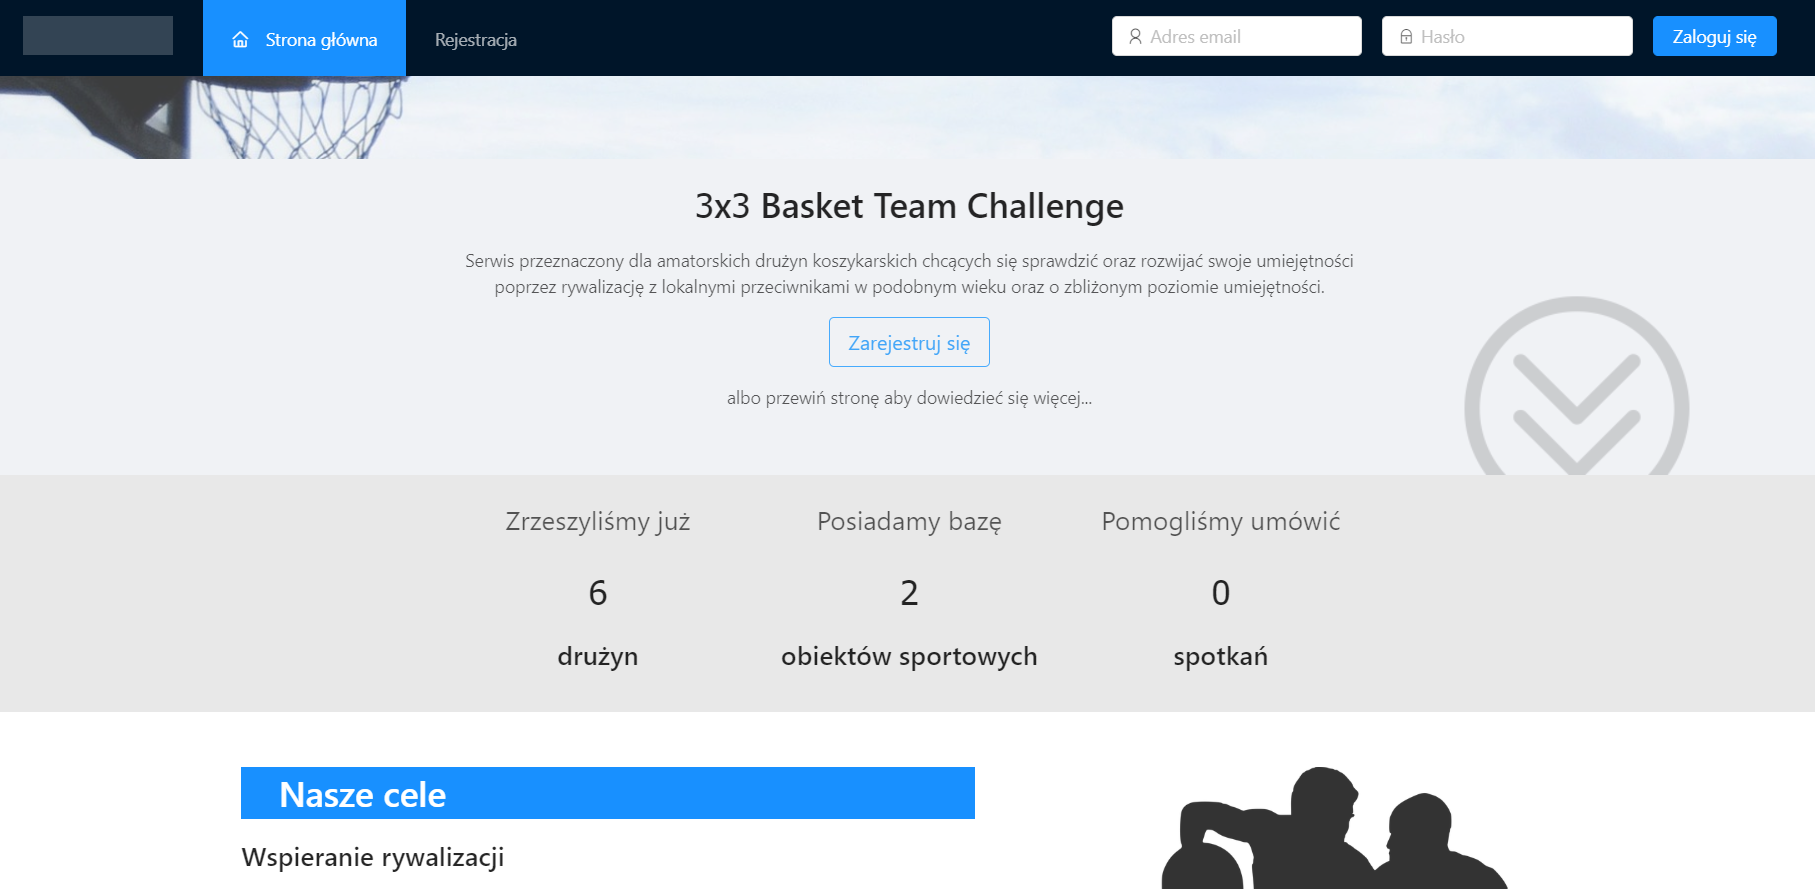
\includegraphics[width=\linewidth]{065-dzialanie/rys/ss-landing.PNG}
\caption{Widok strony głównej systemu}
\label{fig:ss-landing}
\end{figure}

Formularz rejestracyjny został przedstawiony na rysunku \ref{fig:ss-register}. Podany przez użytkownika adres e-mail będzie jego loginem do systemu. Hasło pobierane jest dwukrotnie w celu zmniejszenia szansy na omyłkowe zadeklarowanie błędnego hasła. Dodatkowo hasło ze względów bezpieczeństwa musi składać się z co najmniej 7 znaków. Imię i nazwisko służy do dalszej identyfikacji użytkownika w systemie. Nowy użytkownik również proszony jest o podanie swojej daty urodzenia, ponieważ wiek zawodników uwzględniany jest podczas dopasowywania drużyn.


\begin{figure}[H]
\centering
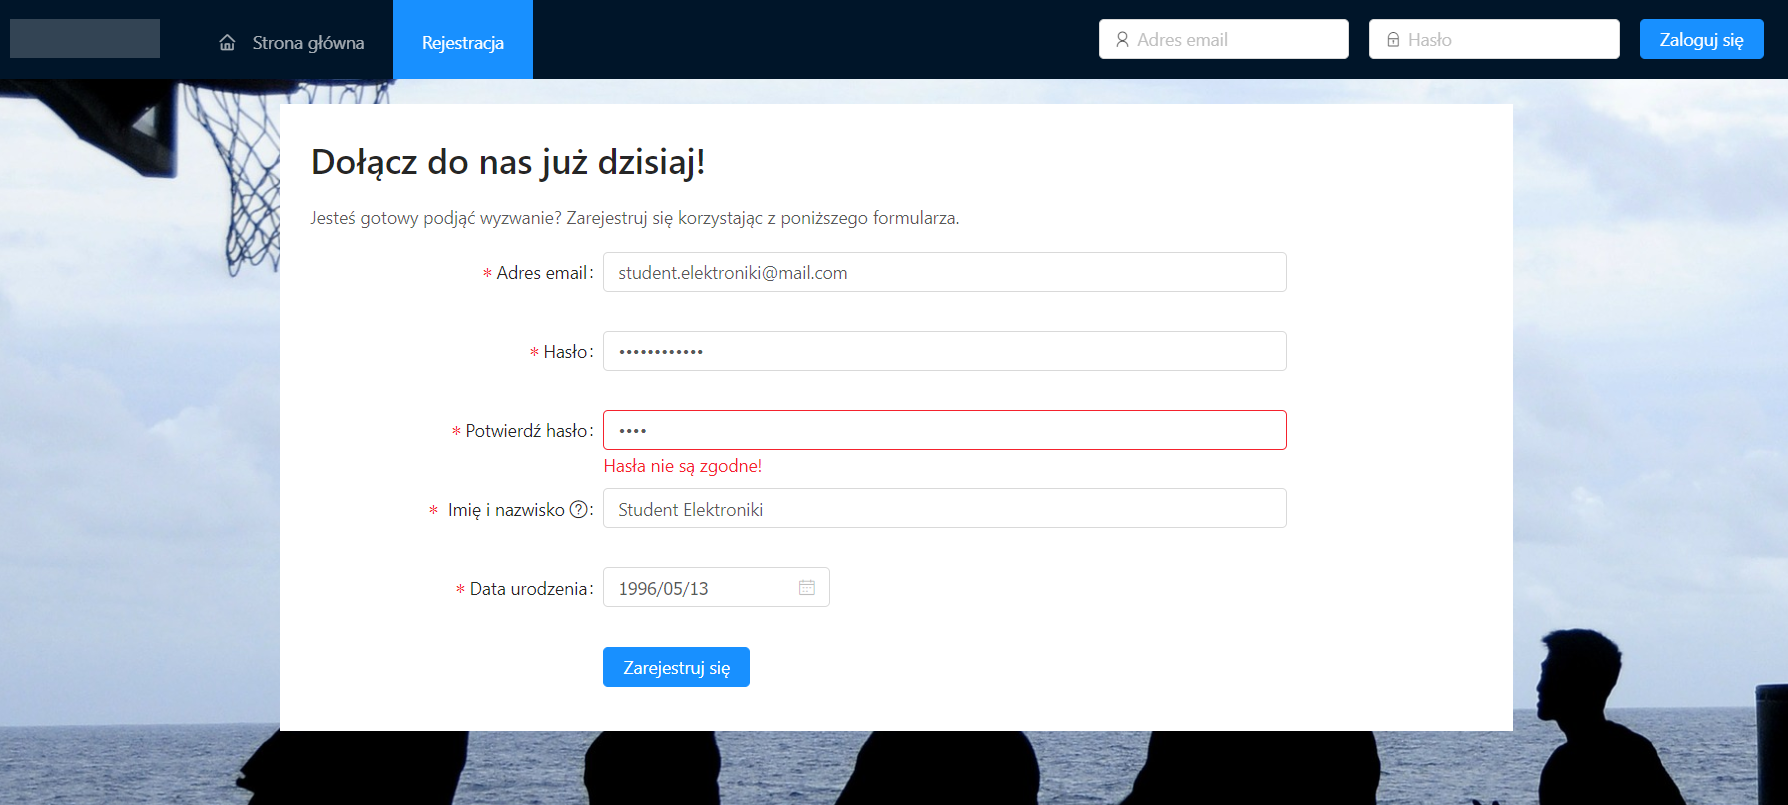
\includegraphics[width=\linewidth]{065-dzialanie/rys/ss-register.PNG}
\caption{Widok formularza rejestracji}
\label{fig:ss-register}
\end{figure}

Po utworzeniu konta użytkownik może się zalogować do systemu za pomocą formularza umieszczonego na pasku nawigacyjnym. Fragment widoku został przedstawiony na rysunku \ref{fig:ss-login}.

\begin{figure}[H]
\centering

\includegraphics[width=\linewidth]{065-dzialanie/rys/ss-login.PNG}
\caption{Widok formularza logowania}
\label{fig:ss-login}
\end{figure}

\section{Tworzenie profilu zawodnika}

Po pierwszym logowaniu nowego użytkownika, zostaje on przekierowany do kreatora zawodnika. Jest to formularz pozwalający na uzupełnienie swojego profilu zawodnika o informacje konieczne dla funkcjonowania systemu Team Challenge. Pierwszy krok formularza przedstawiono na rysunku \ref{fig:ss-profile-1}.


\begin{figure}[H]
\centering
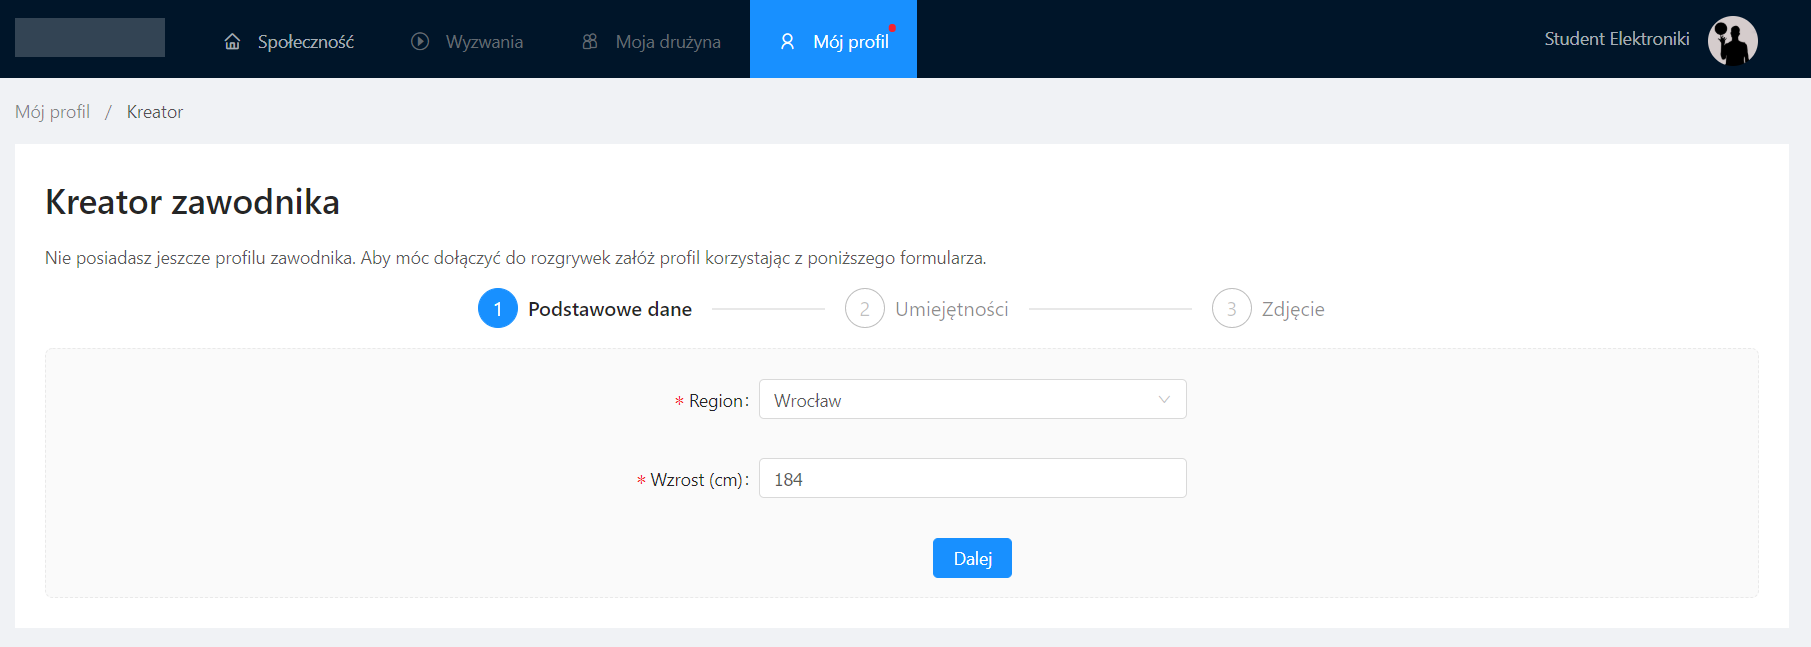
\includegraphics[width=\linewidth]{065-dzialanie/rys/ss-profile-1.PNG}
\caption{Widok kreatora zawodnika - krok 1}
\label{fig:ss-profile-1}
\end{figure}

Region jest wybierany spośród zdefiniowanych przez administratora. W prototypowej wersji systemu są to Wrocław oraz Kłodzko. Zawodnik proszony jest o wprowadzenie swojego wzrostu, jednak ta cecha nie ma wpływu na działanie systemu. Najistotniejsze informacje z punktu widzenia mechanizmu dopasowywania pobierane są w drugim kroku formularza, który przedstawiono na rysunku \ref{fig:ss-profile-2}.

\begin{figure}[H]
\centering
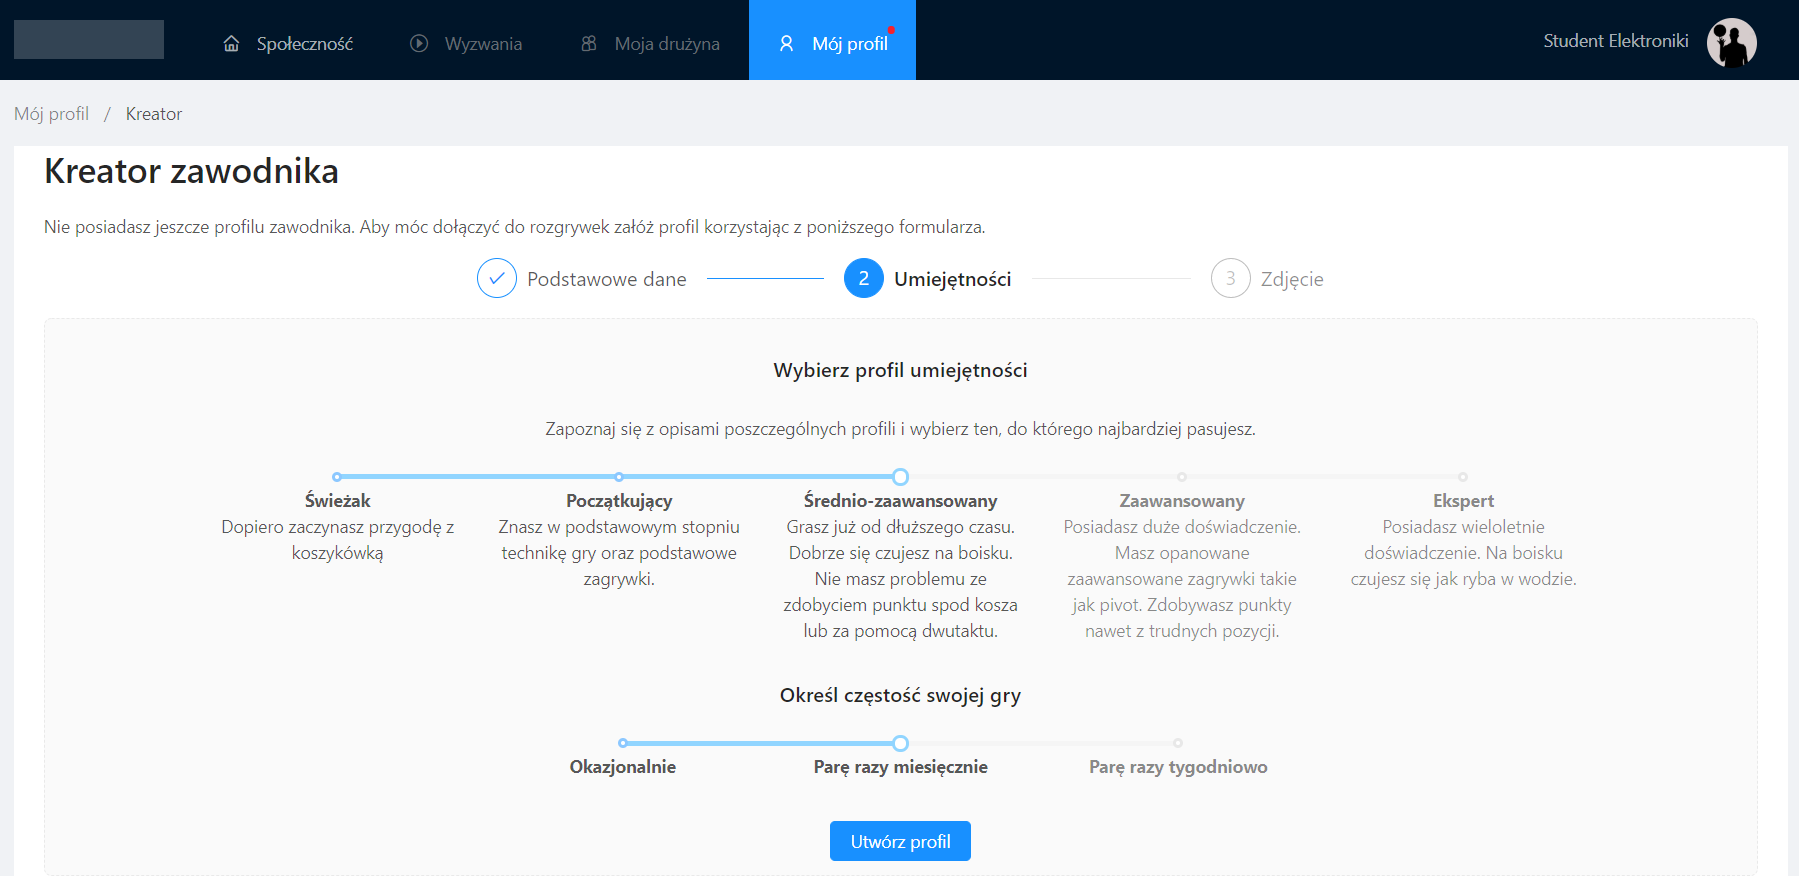
\includegraphics[width=\linewidth]{065-dzialanie/rys/ss-profile-2.PNG}
\caption{Widok kreatora zawodnika - krok 2}
\label{fig:ss-profile-2}
\end{figure}

Użytkownik deklaruje swój stopień zaawansowania oraz częstość gry. Na podstawie tych dwóch wartości system przypisuje zawodnikowi wartość w zakresie 0 do 10 określającą jego umiejętności z uwzględnieniem aktualnej formy. Wartość ta steruje kryterium bliskiego poziomu umiejętności zawodników podczas dopasowywania. Ostatni krok formularza jest w pełni opcjonalny, pozwala on na wgranie do systemu zdjęcia lub awatara - rysunek \ref{fig:ss-profile-3}.

\begin{figure}[H]
\centering
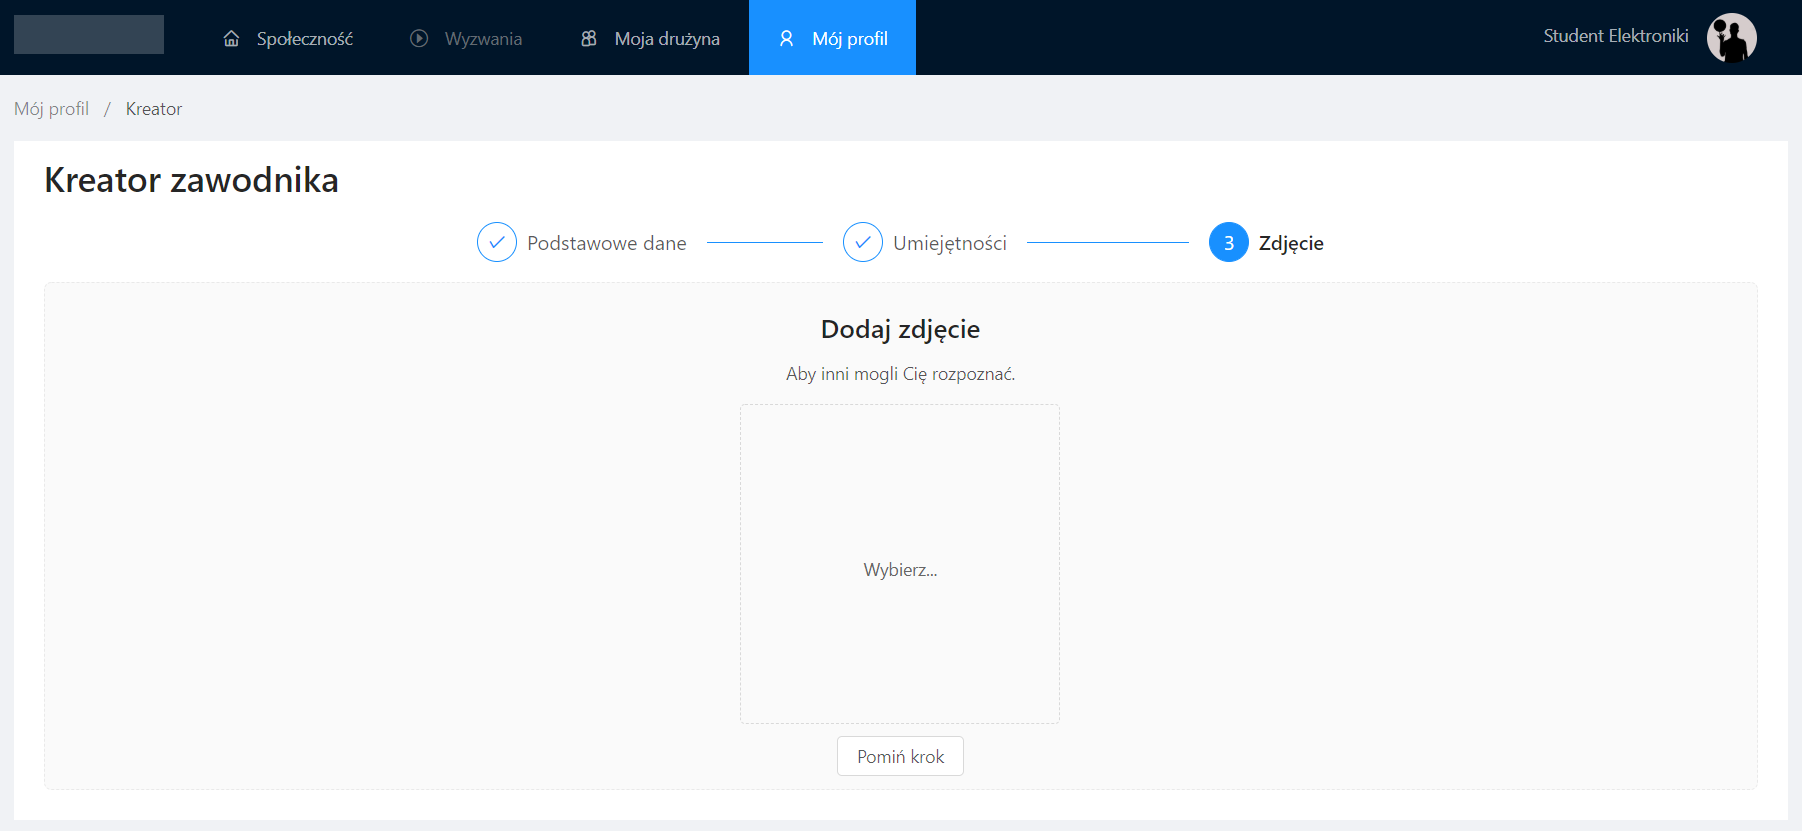
\includegraphics[width=\linewidth]{065-dzialanie/rys/ss-profile-3.PNG}
\caption{Widok kreatora zawodnika - krok 3}
\label{fig:ss-profile-3}
\end{figure}

Na rysunku \ref{fig:ss-profile-ready} przedstawiono utworzony profil zawodnika. Ukazany awatar jest domyślny dla wszystkich zawodników, którzy nie wgrali własnego zdjęcia.

\begin{figure}[H]
\centering
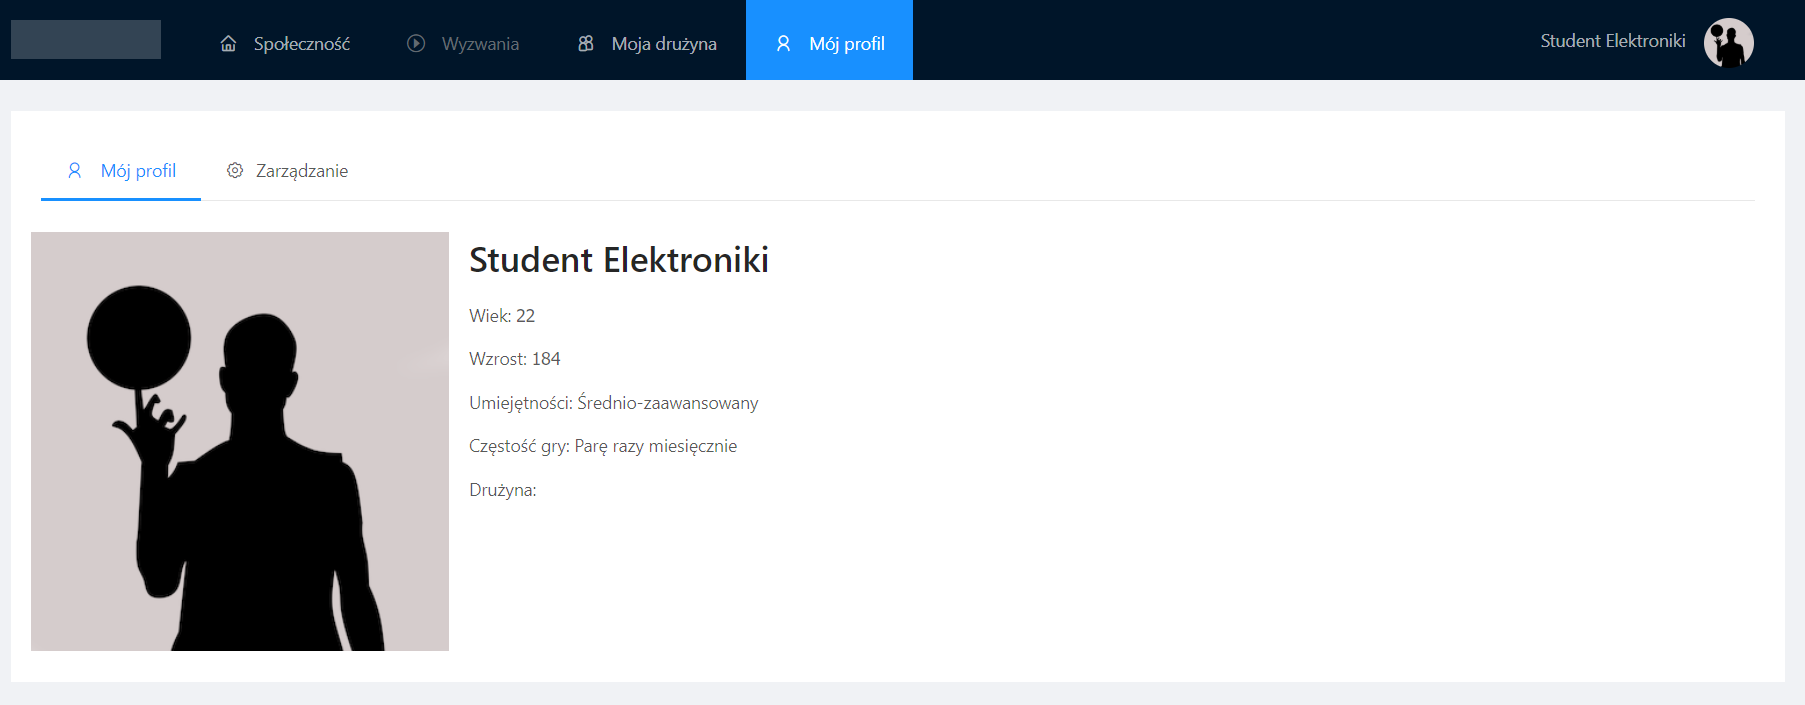
\includegraphics[width=\linewidth]{065-dzialanie/rys/ss-profile-ready.PNG}
\caption{Widok profilu zawodnika}
\label{fig:ss-profile-ready}
\end{figure}

\section{Tworzenie drużyny}
Funkcjonalność tworzenia drużyny znajduje się pod przyciskiem ``Załóż drużynę`` widocznym w zakładce ``Moja drużyna`` gdy zawodnik nie należy do żadnej drużyny, co ukazano na rysunku \ref{fig:ss-team-no}.

\begin{figure}[H]
\centering
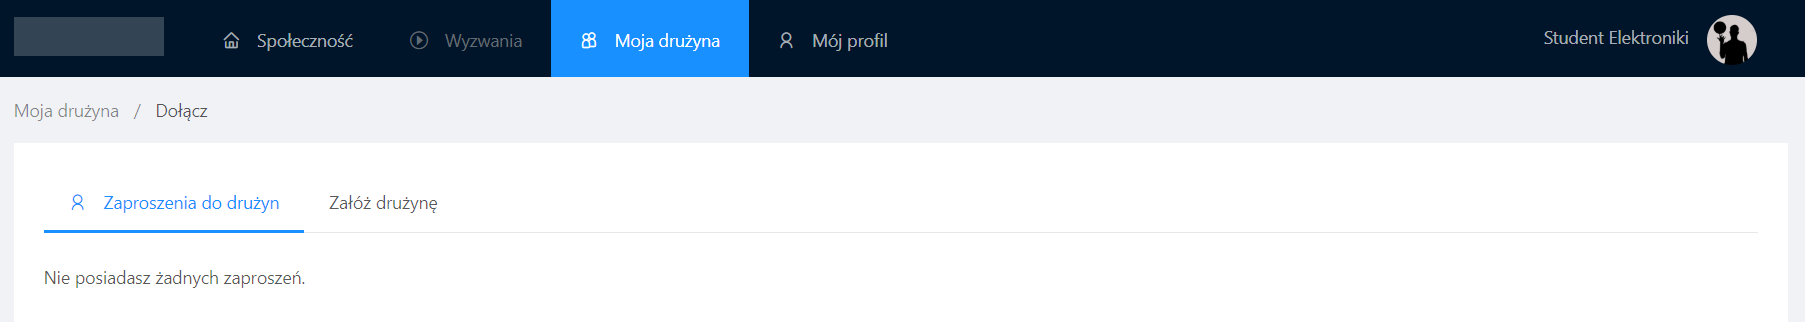
\includegraphics[width=\linewidth]{065-dzialanie/rys/ss-team-no.PNG}
\caption{Widok zakładki ``Moja drużyna``}
\label{fig:ss-team-no}
\end{figure}

Pierwszym krokiem jest zdefiniowanie nazwy drużyny. Nazwa ta będzie reprezentować drużynę w systemie. Region drużyny wybierany jest automatycznie na podstawie regionu wybranego przez zawodnika podczas tworzenia profilu.


\begin{figure}[H]
\centering
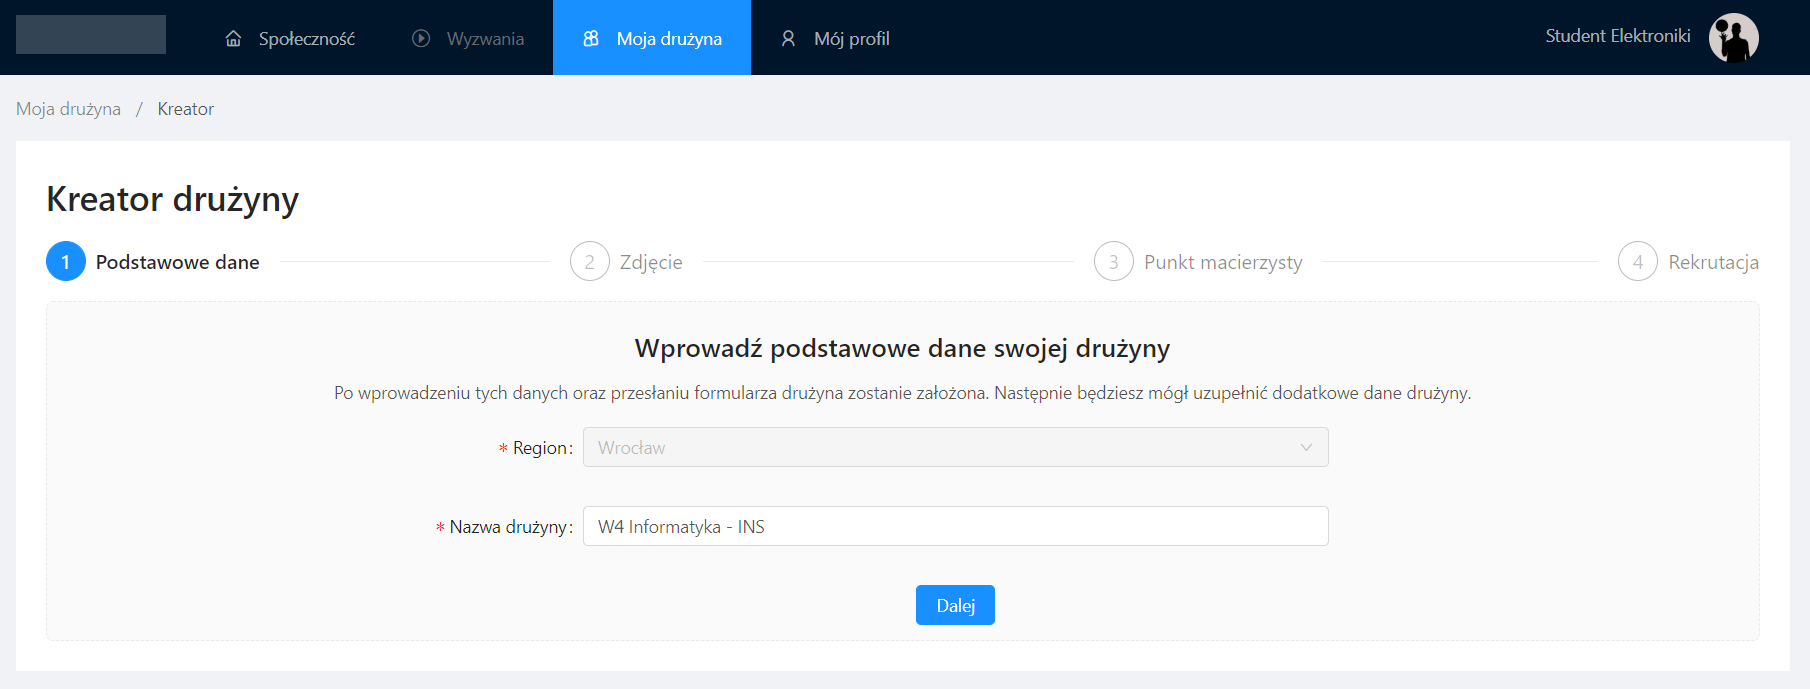
\includegraphics[width=\linewidth]{065-dzialanie/rys/ss-team-1.PNG}
\caption{Widok kreatora drużyny - krok 1}
\label{fig:ss-team-1}
\end{figure}

Podobnie jak w przypadku profilu zawodnika, kapitan ma możliwość wgrania zdjęcia drużyny. Widok po wgraniu przykładowego zdjęcia przedstawiono na rysunku \ref{fig:ss-team-2}.

\begin{figure}[H]
\centering
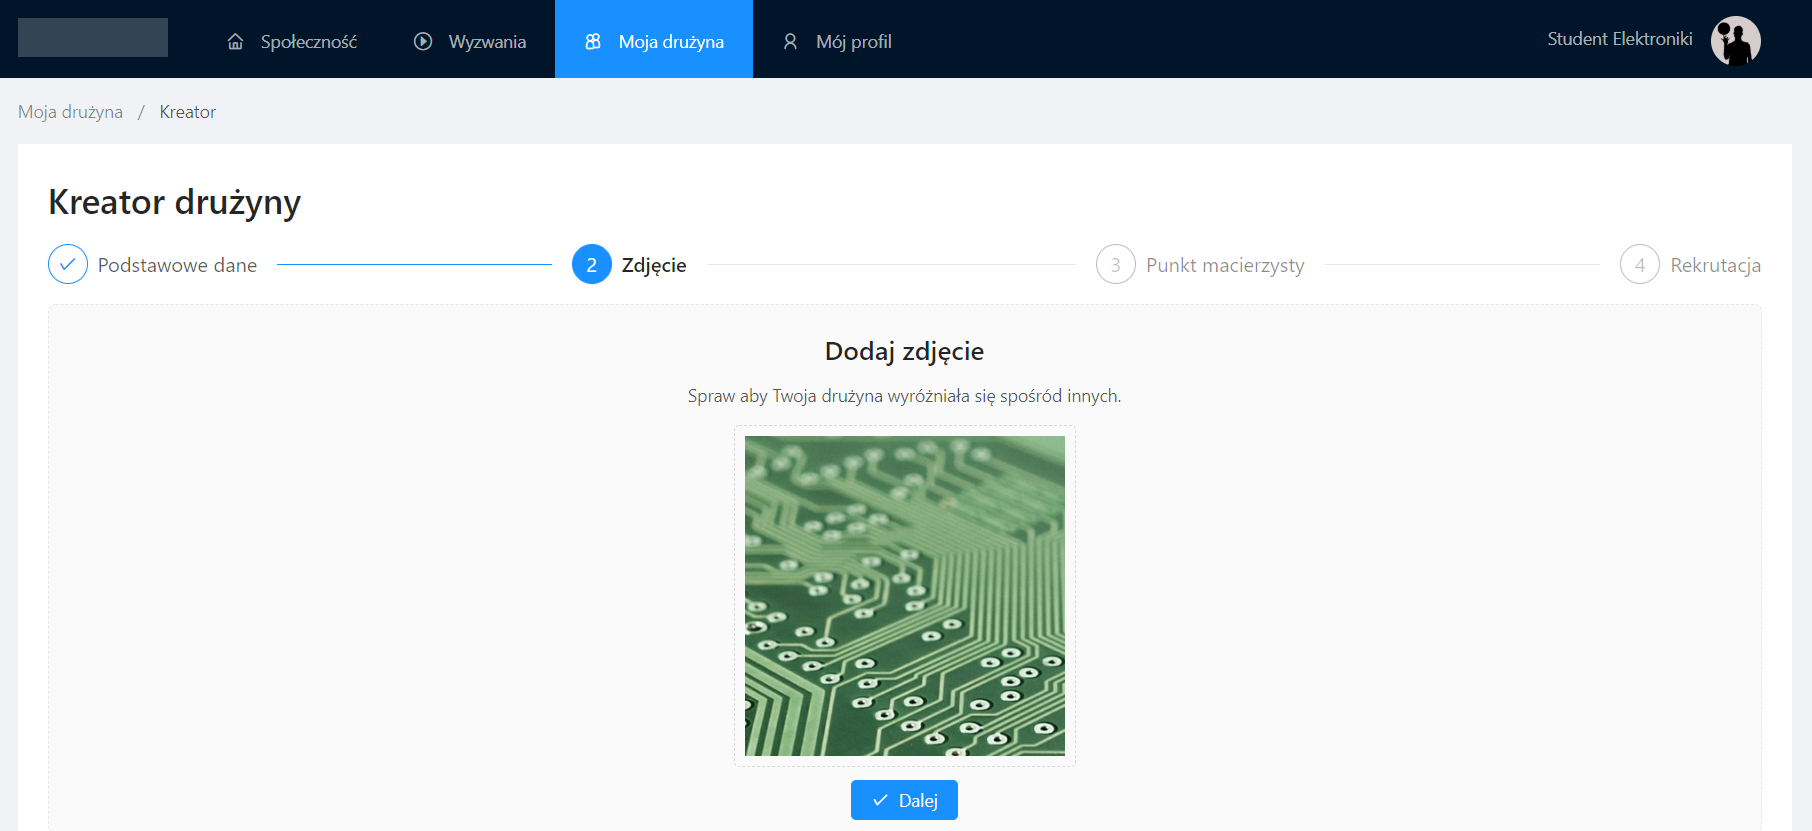
\includegraphics[width=\linewidth]{065-dzialanie/rys/ss-team-2.PNG}
\caption{Widok kreatora drużyny - krok 2}
\label{fig:ss-team-2}
\end{figure}

Kapitan może wybrać punkt macierzysty drużyny, czyli lokalizację służącą do porównań odległości między drużynami. W tym celu użytkownik może przemieszczać zielony marker na mapie poprzez wciskanie docelowych punktów. Domyślnie jest to centrum regionu, jednak zalecane jest ustawienie miejsca, które jest pobliskie zawodnikom. W przypadku studentów elektroniki mieszkających w okolicy kampusu może to być budynek wydziału. Przykładowe ustawienie zaprezentowano na rysunku \ref{fig:ss-team-3}. 

\begin{figure}[H]
\centering
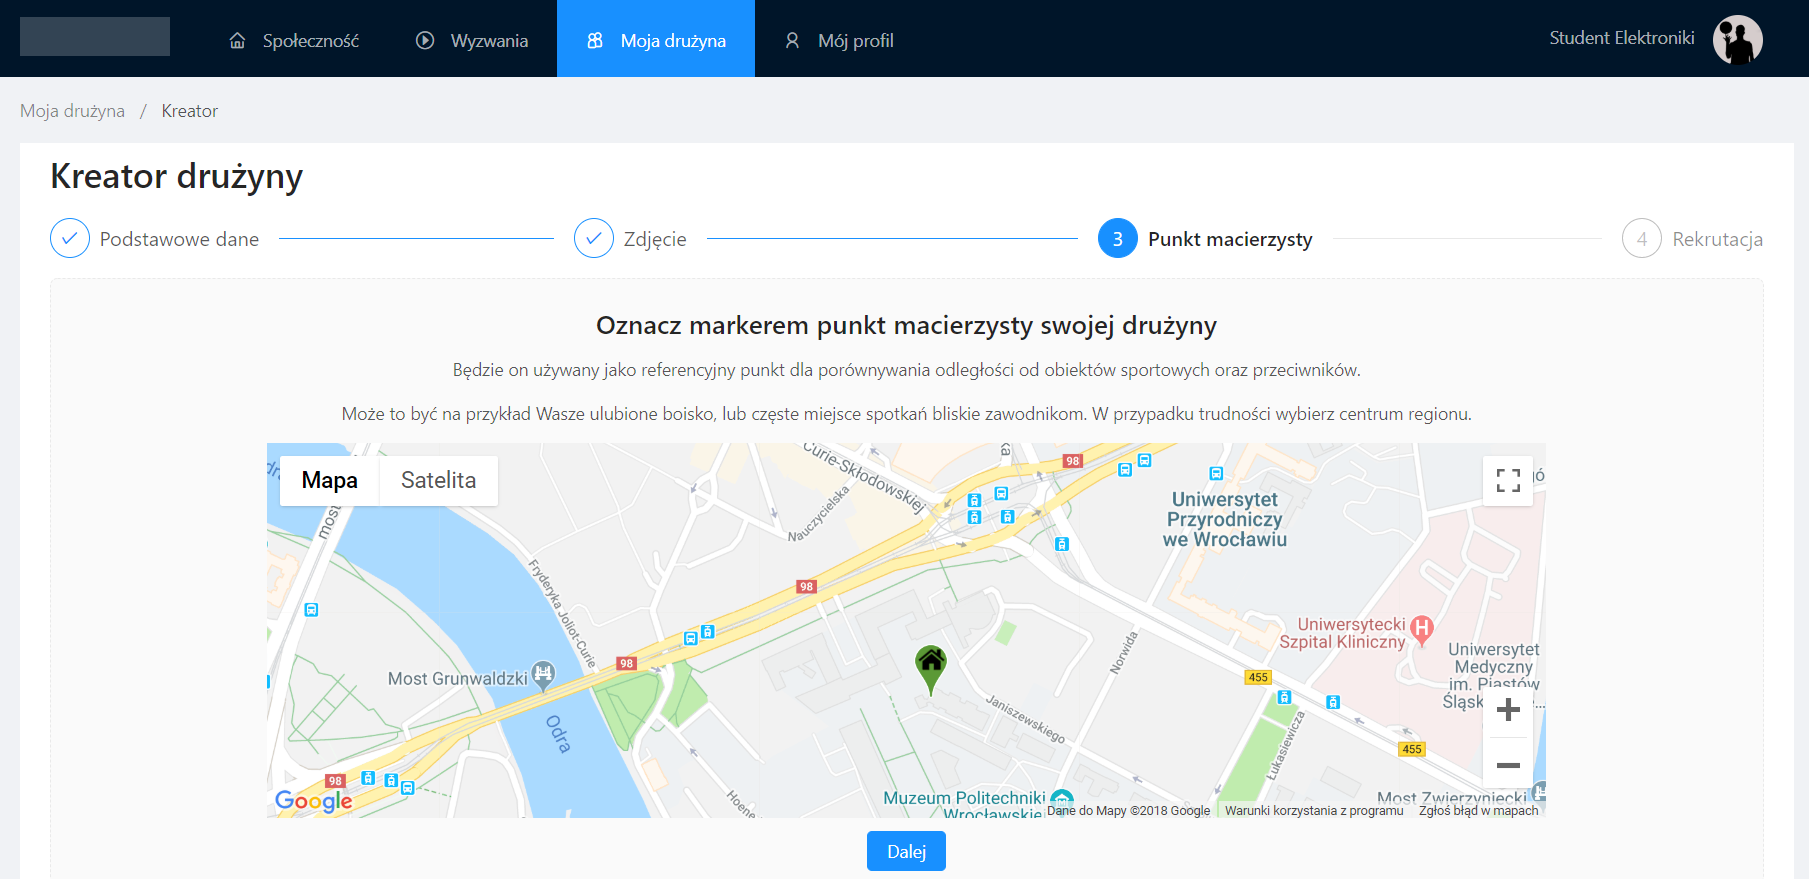
\includegraphics[width=\linewidth]{065-dzialanie/rys/ss-team-3.PNG}
\caption{Widok kreatora drużyny - krok 3}
\label{fig:ss-team-3}
\end{figure}

Ostatnim krokiem kreatora jest widok rekrutacji, który umożliwia wysłanie wstępnych zaproszeń zawodników do drużyny. Zawodnicy są przedstawieni w tabeli z możliwością ich wyszukiwania po imieniu oraz nazwisku. Tabela przedstawia jedynie zawodników, których można zaprosić, czyli zdefiniowanych dla tego samego regionu co drużyna oraz nie będący w innym zespole. Widok przedstawiono na rysunku \ref{fig:ss-team-5}.

\begin{figure}[H]
\centering
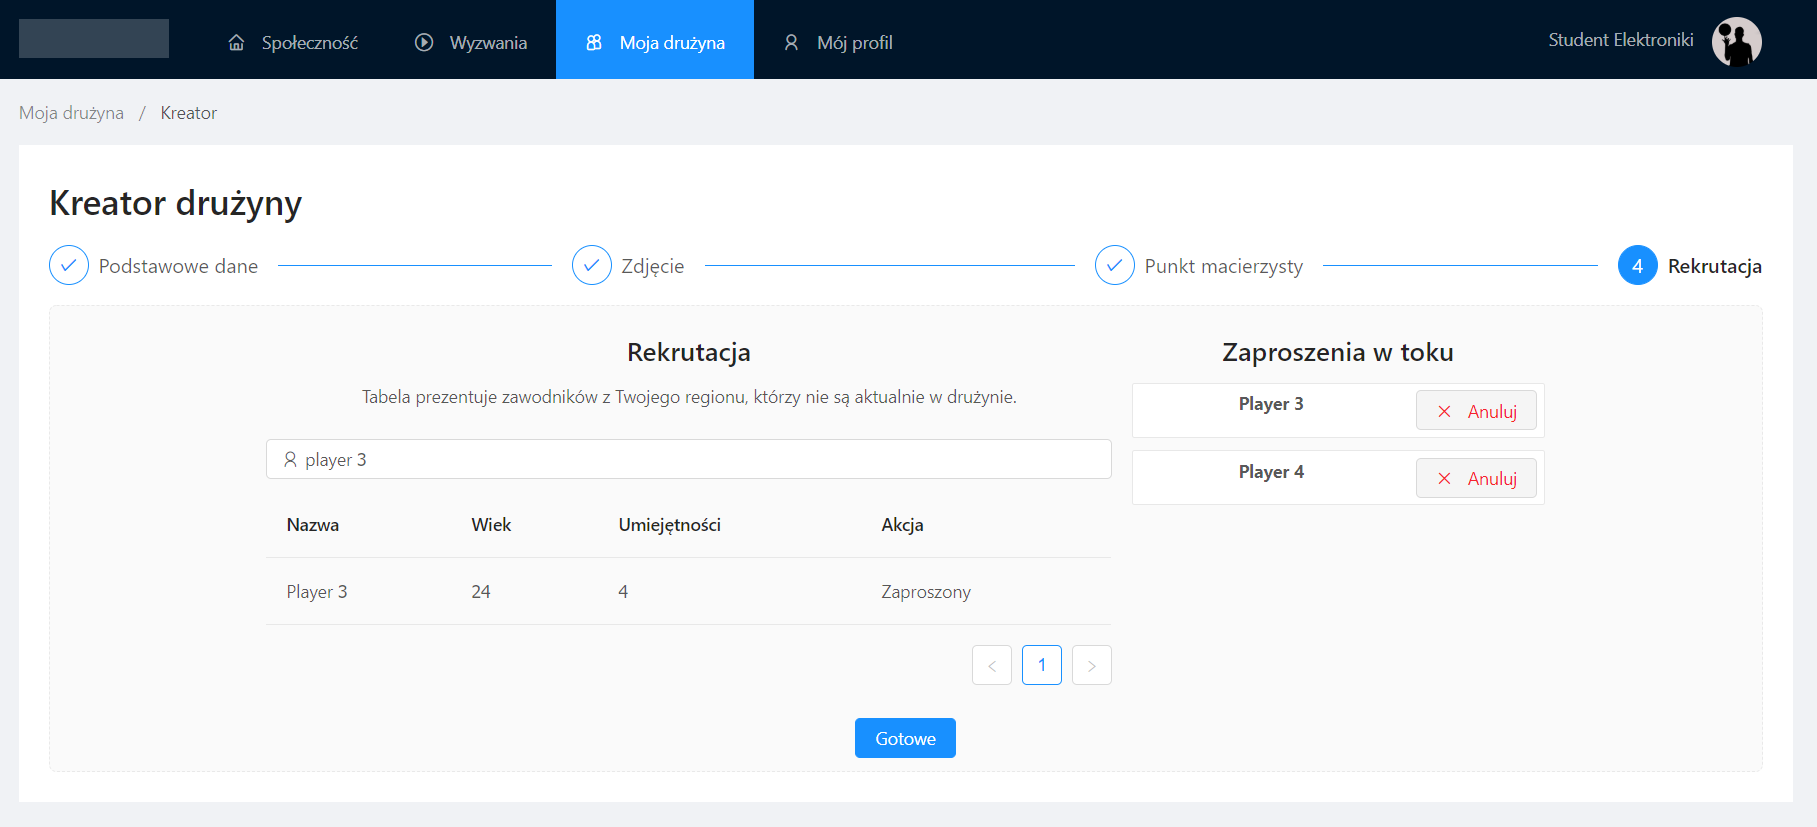
\includegraphics[width=\linewidth]{065-dzialanie/rys/ss-team-5.PNG}
\caption{Widok kreatora drużyny - krok 4}
\label{fig:ss-team-5}
\end{figure}

\section{Wyszukiwanie rywali i rzucanie wyzwań}

Funkcjonalność wyszukiwania rywali oraz umawiania spotkań staje się dostępna dla kapitana drużyny w momencie gdy zbierze on co najmniej trzech zawodników. Jest to minimalny rozmiar drużyny dla koszykówki 3 na 3. Kapitan aktywnej drużyny ma dostęp do przycisku ``Szukaj rywali`` na pasku nawigacji. Przycisk ten służy do szybkiej nawigacji do funkcjonalności z każdego miejsca aplikacji. Kapitan może również użyć zakładki ``Szukaj rywali`` w widoku społeczności, który widoczny jest na rysunku \ref{fig:ss-search-0}. 

\begin{figure}[H]
\centering
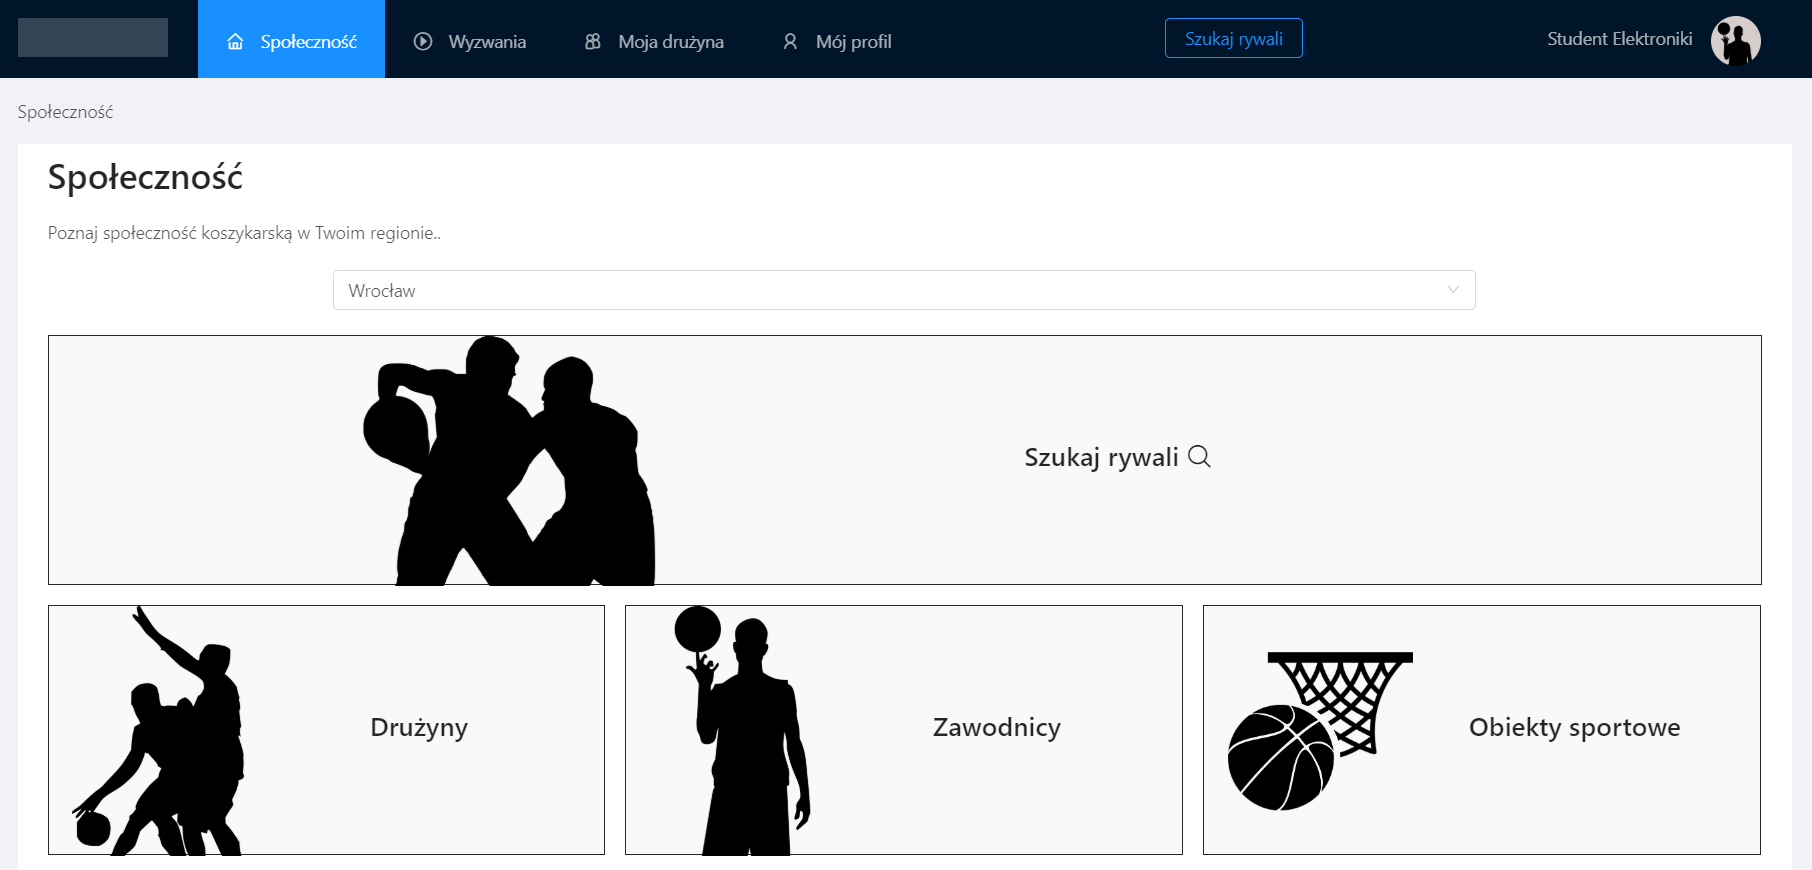
\includegraphics[width=\linewidth]{065-dzialanie/rys/ss-search-0.PNG}
\caption{Widok zakładki ``Społeczność``}
\label{fig:ss-search-0}
\end{figure}

Pierwszym etapem wyszukiwania rywali jest określenie preferencji kapitana. Formularz został przedstawiony na rysunku \ref{fig:ss-search-1}. Zadaniem kapitana jest rozdysponowanie 100 punktów preferencji pomiędzy cechy rywali takie jak: podobny wiek, podobne doświadczenie oraz mała odległość między punktami macierzystymi. Podział pomiędzy te trzy cechy odbywa się za pomocą suwaków, które zostały skonstruowane tak, aby ich wartości w sumie zawsze dawały 100. Oznacza to, że zwiększając wartość jednego suwaka, zmniejszamy wartość dwóch pozostałych. Kapitan może zablokować wybrany suwak na określonej wartości za pomocą symbolu kłódki znajdującej się po lewej stronie. Po prawej stronie ekranu znajdują się także dodatkowe preferencje takie jak poziom fair-play, ponowne spotkanie oraz duża aktywność przeciwników. Na podstawie wypełnionego formularza obliczane są wagi poszczególnych kryteriów dla algorytmu optymalizacji wielokryterialnej. Proporcje między wartościami punktów preferencji dla poszczególnych cech przekształcane są na wagi kryteriów liczbowych, a zadeklarowane dodatkowe preferencje powodują uwzględnianie w ocenie poszczególnych drużyn wybranych kryteriów logicznych (rozdział 6.2.6). 




\begin{figure}[H]
\centering
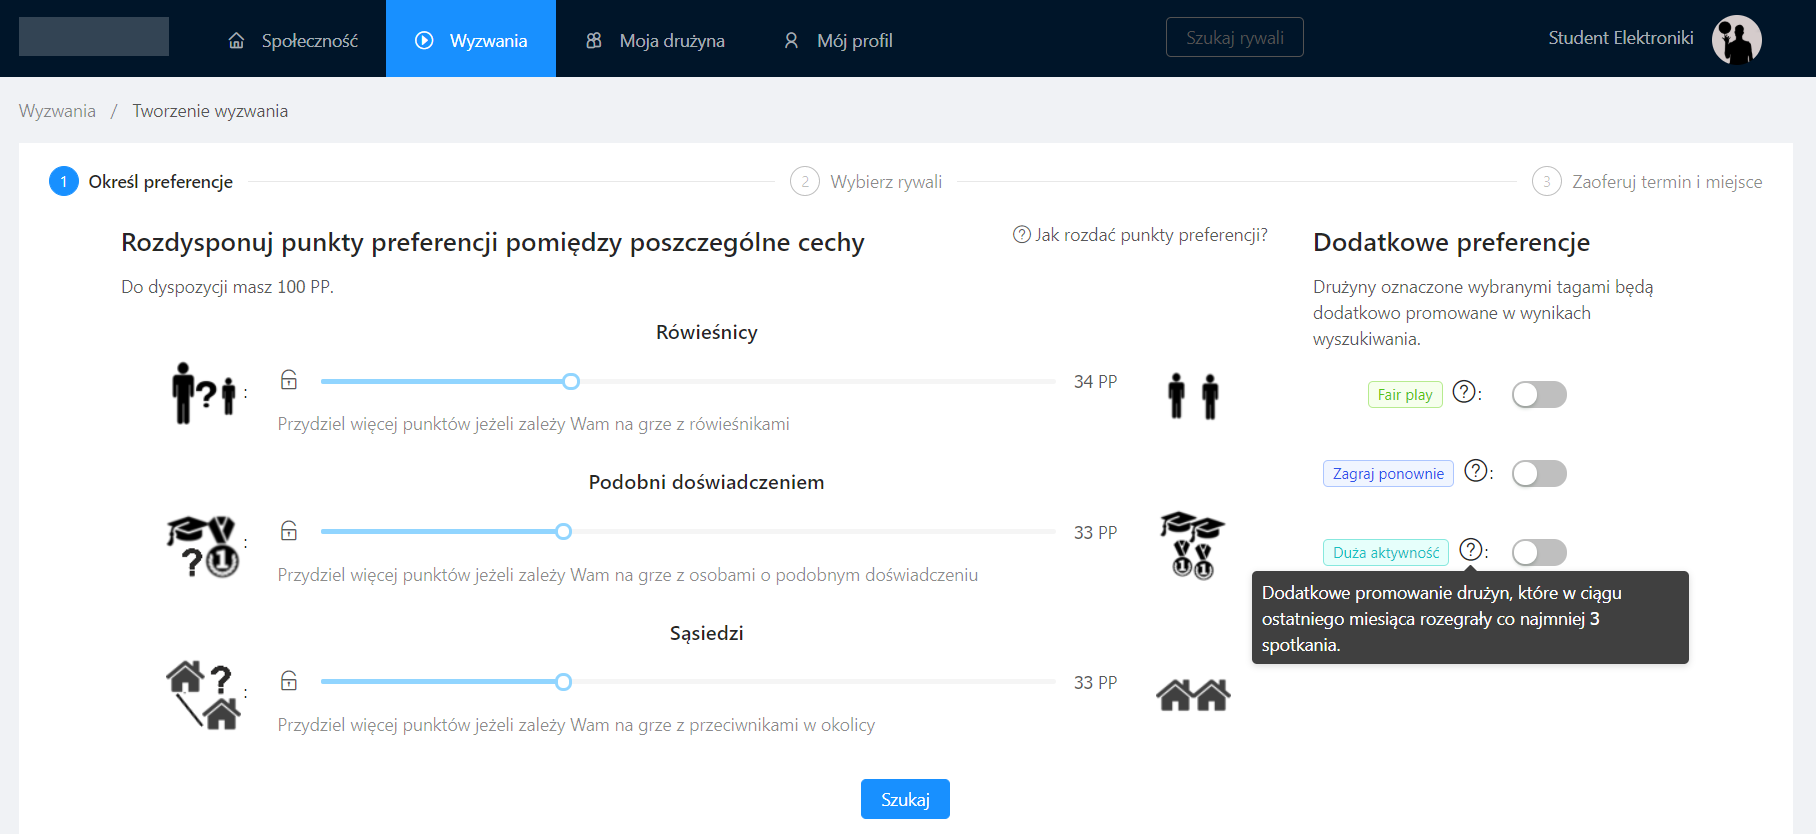
\includegraphics[width=\linewidth]{065-dzialanie/rys/ss-search-1.PNG}
\caption{Widok formularza deklaracji preferencji drużyny}
\label{fig:ss-search-1}
\end{figure}

Wyniki wyszukiwania przedstawione są w postaci listy posortowanej według poziomu dopasowania. Poziom dopasowania jest oceną ważoną poszczególnych drużyn z uwzględnieniem preferencji kapitana. Dla każdej z drużyn wyświetlane są znaczniki, które odpowiadają cechom związanymi z dodatkowymi preferencjami oraz poziomy dopasowań pod względem wieku, umiejętności oraz odległości. Przykładowy widok przedstawiono na rysunku \ref{fig:ss-search-2}.    


\begin{figure}[H]
\centering
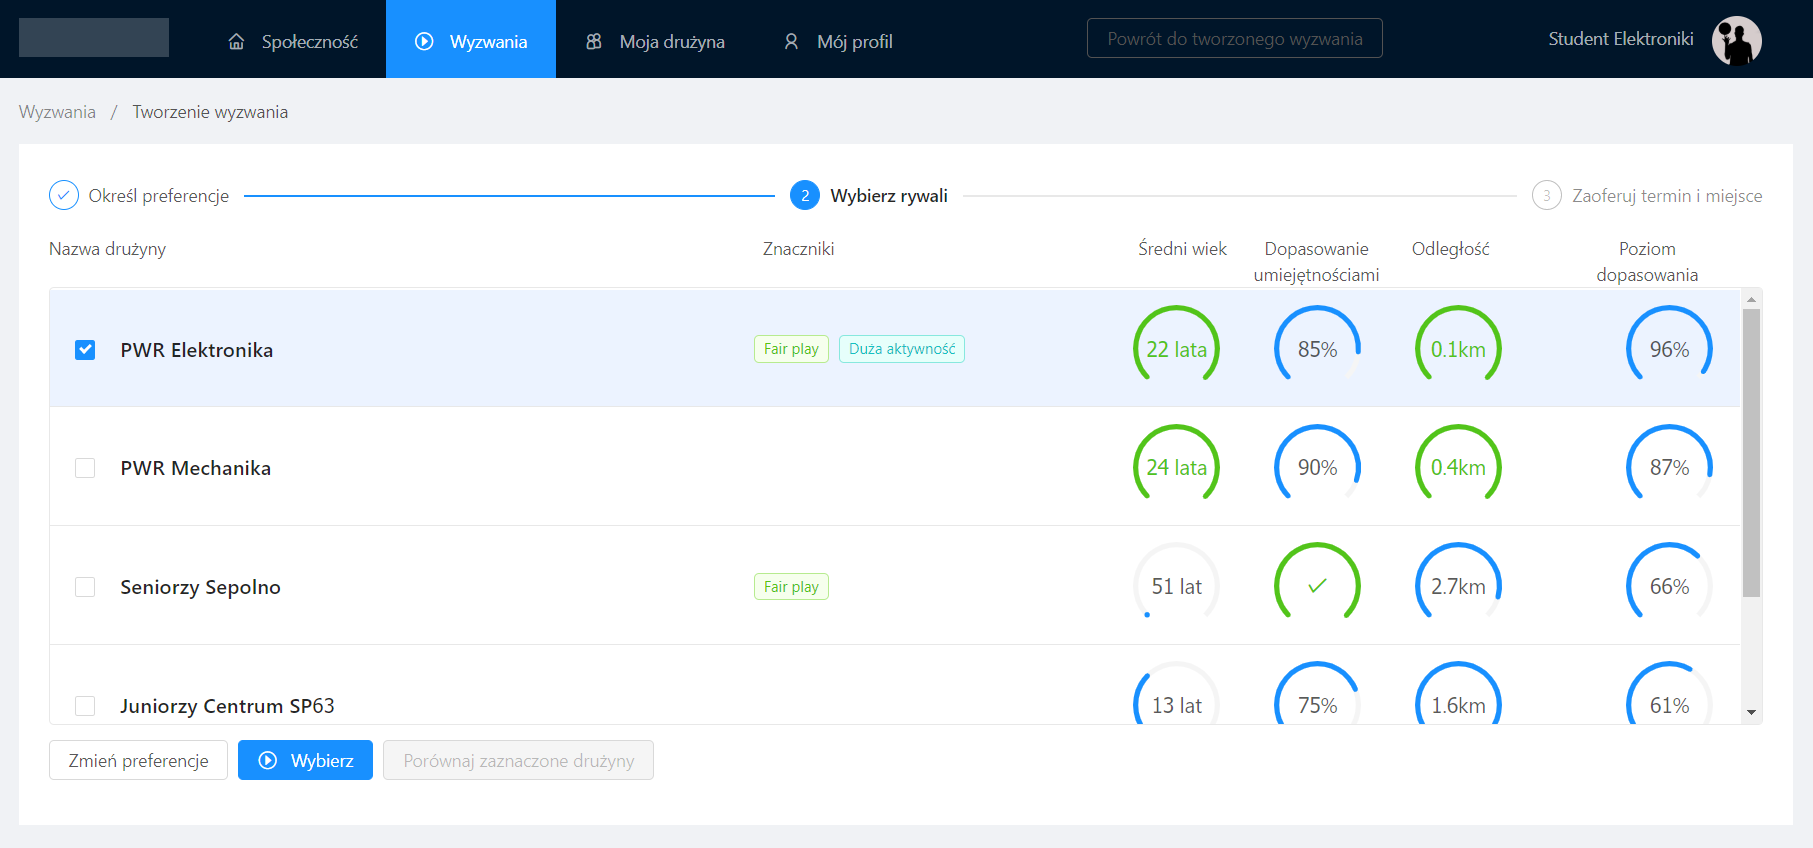
\includegraphics[width=\linewidth]{065-dzialanie/rys/ss-search-2.PNG}
\caption{Widok wyników wyszukiwania rywali}
\label{fig:ss-search-2}
\end{figure}

Kapitan wnioskując na podstawie wskaźników może od razu wybrać rywali albo zaznaczyć dwie lub trzy drużyny w celu porównania. W momencie zaznaczenia odpowiedniej liczby elementów uaktywnia się przycisk "Porównaj zaznaczone drużyny", który przenosi użytkownika do widoku porównania przedstawionego na rysunku \ref{fig:ss-search-4}. Wybrane drużyny zostają zestawione w sąsiednich kolumnach w celu ułatwienia podjęcia decyzji kapitanowi. Wykres przedstawia dopasowanie poszczególnych drużyn, a na mapie znajdują się punkty macierzyste zespołu kapitana oraz pozostałych będących porównywanych. W dolnej części widoku nie ujętej na zrzucie ekranu znajdują się informacje w formie tekstowej oraz przedstawieni są zawodnicy poszczególnych zespołów.

\begin{figure}[H]
\centering
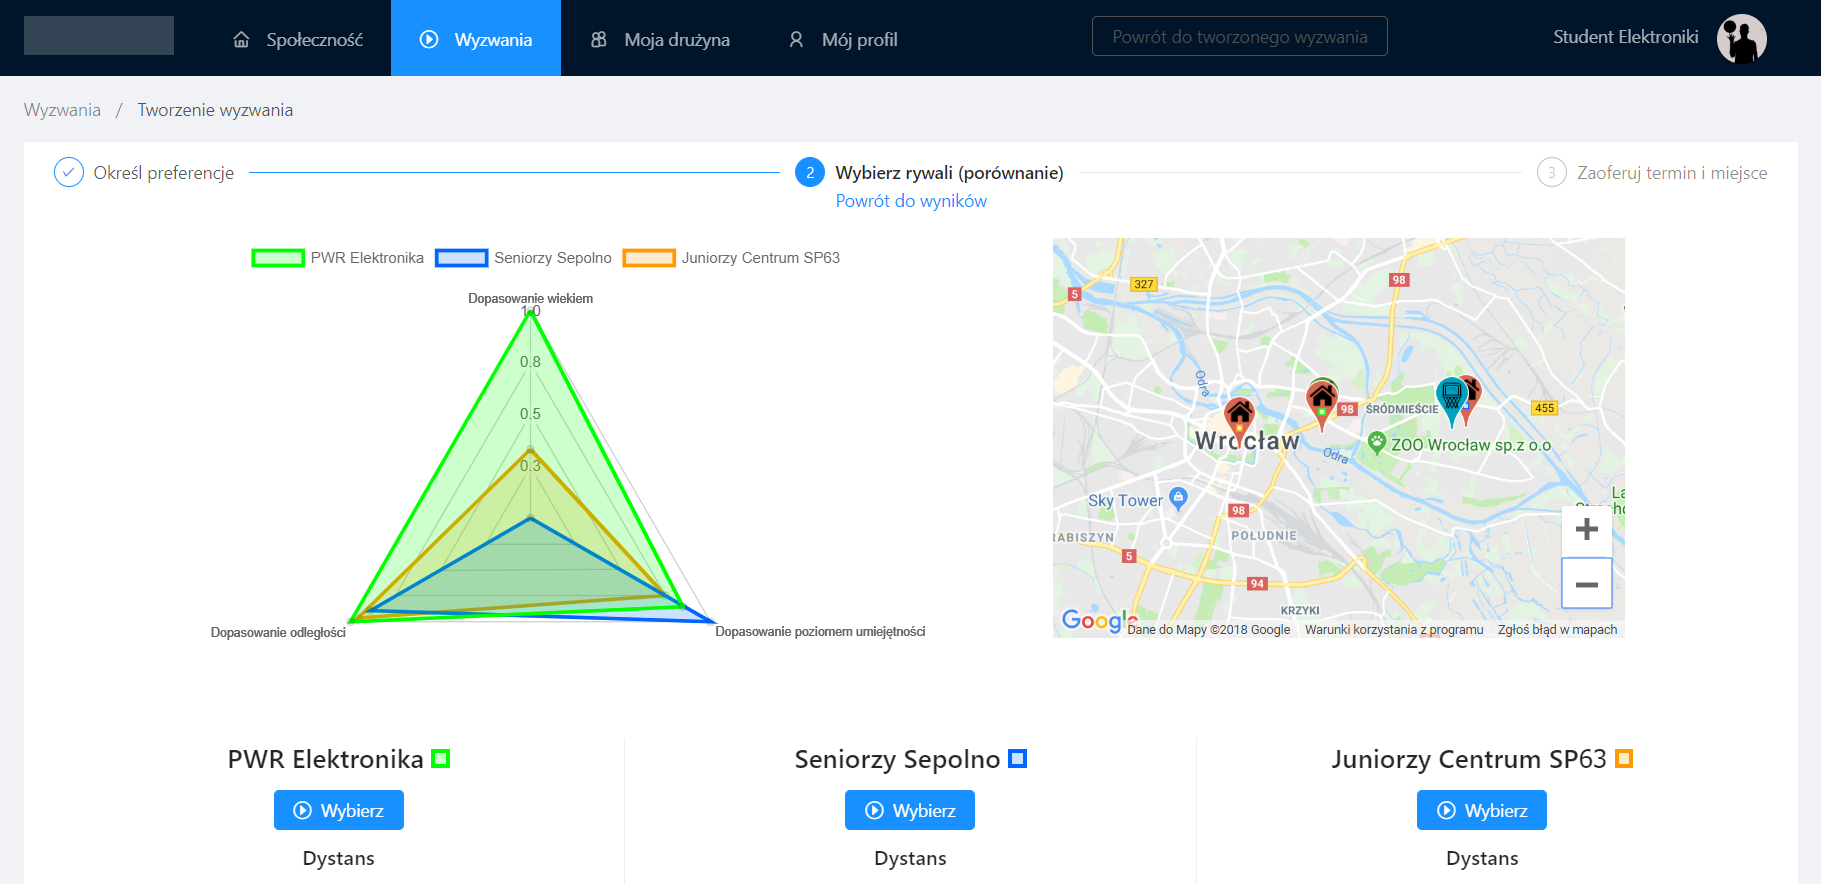
\includegraphics[width=\linewidth]{065-dzialanie/rys/ss-search-4.PNG}
\caption{Widok porównania potencjalnych rywali}
\label{fig:ss-search-4}
\end{figure}

Na potrzeby przykładu wybrana została drużyna PWR Elektronika, która jest bardzo dobrze dopasowana do drużyny poszukującej. Następnym krokiem jest rzucenie wyzwania za pomocą widoku przedstawionego na rysunku \ref{fig:ss-search-5}. Kapitan musi dodać co najmniej jedną ofertę czasu oraz miejsca spotkania za pomocą bloku ``+Nowa oferta``. Formularz wprowadzania oferty przedstawiono na rysunku \ref{fig:ss-search-6}.

\begin{figure}[H]
\centering
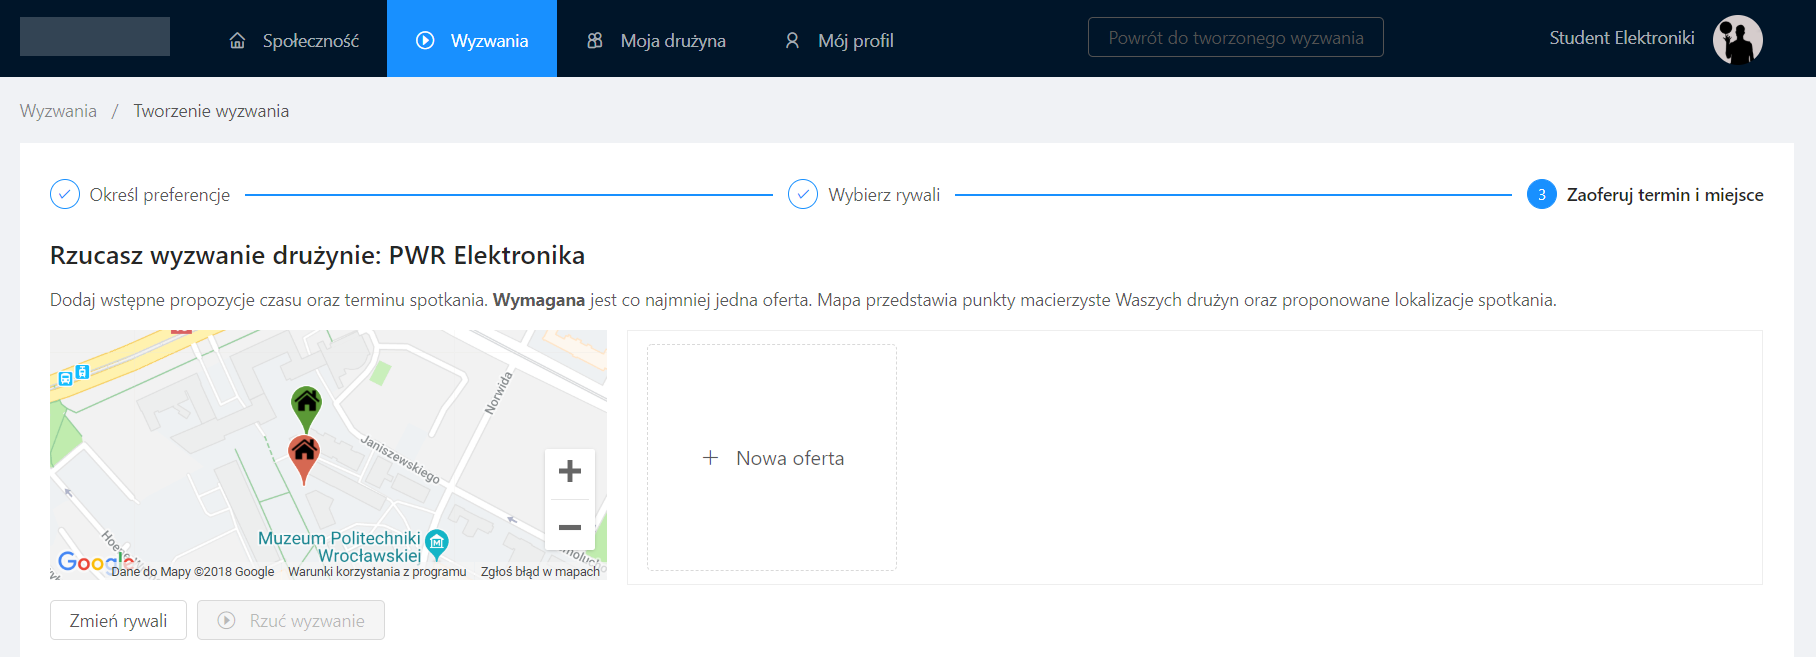
\includegraphics[width=\linewidth]{065-dzialanie/rys/ss-search-5.PNG}
\caption{Widok puli wstępnych ofert czasu oraz miejsca spotkania}
\label{fig:ss-search-5}
\end{figure}


\begin{figure}[H]
\centering
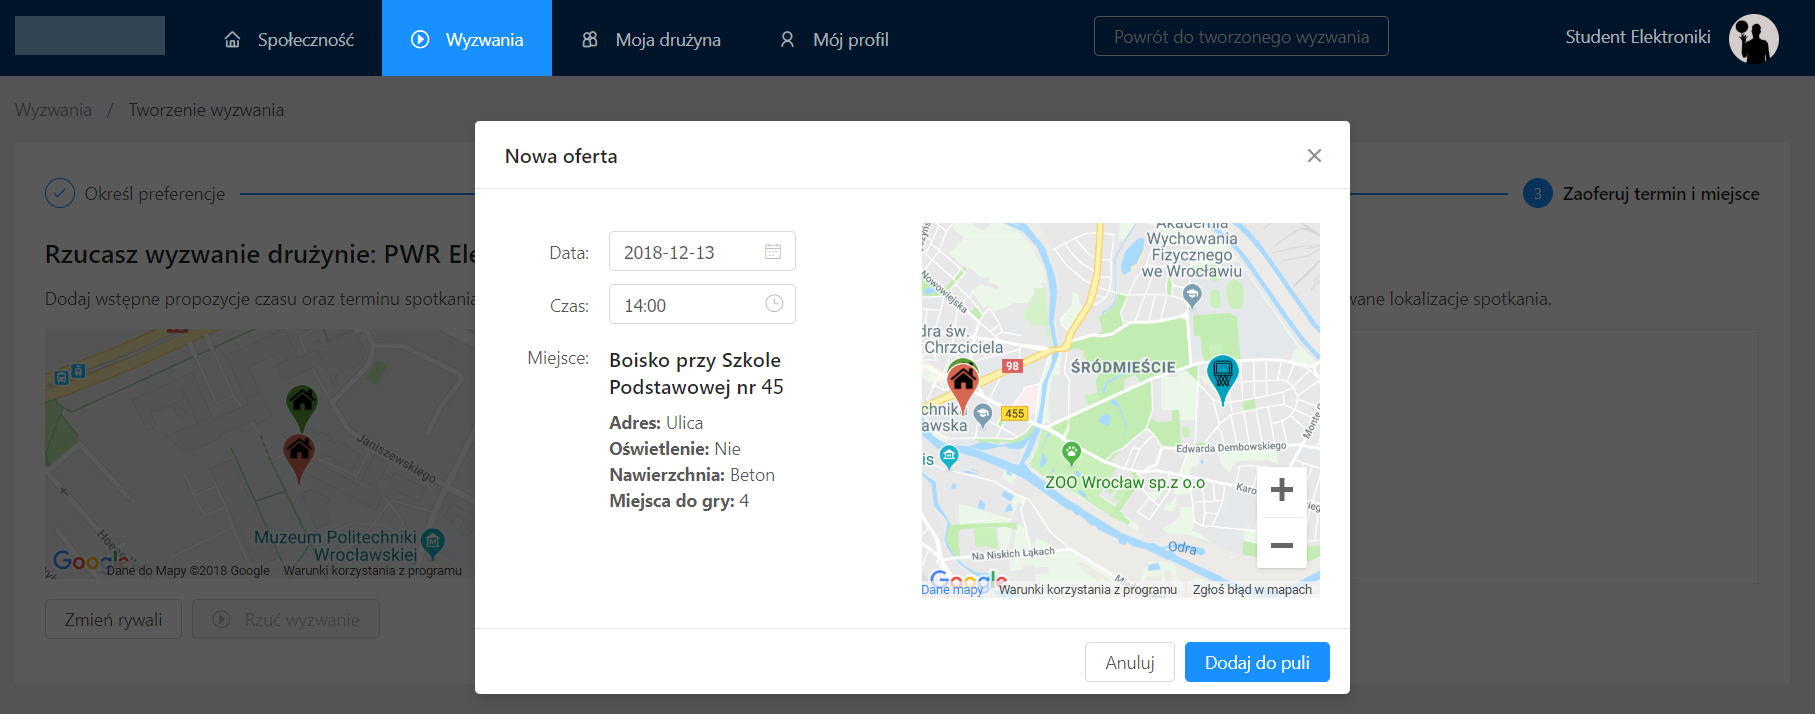
\includegraphics[width=\linewidth]{065-dzialanie/rys/ss-search-6.PNG}
\caption{Widok formularza tworzenia nowej oferty czasu i miejsca spotkania}
\label{fig:ss-search-6}
\end{figure}

Wprowadzone oferty widoczne są w puli, jak na rysunku \ref{fig:ss-search-6}. Kapitan ma możliwość wycofania ofert przy użyciu przycisku ``Anuluj``. W momencie wprowadzenia co najmniej jednej oferty przycisk ``Rzuć wyzwanie`` uaktywnia się.


\begin{figure}[H]
\centering
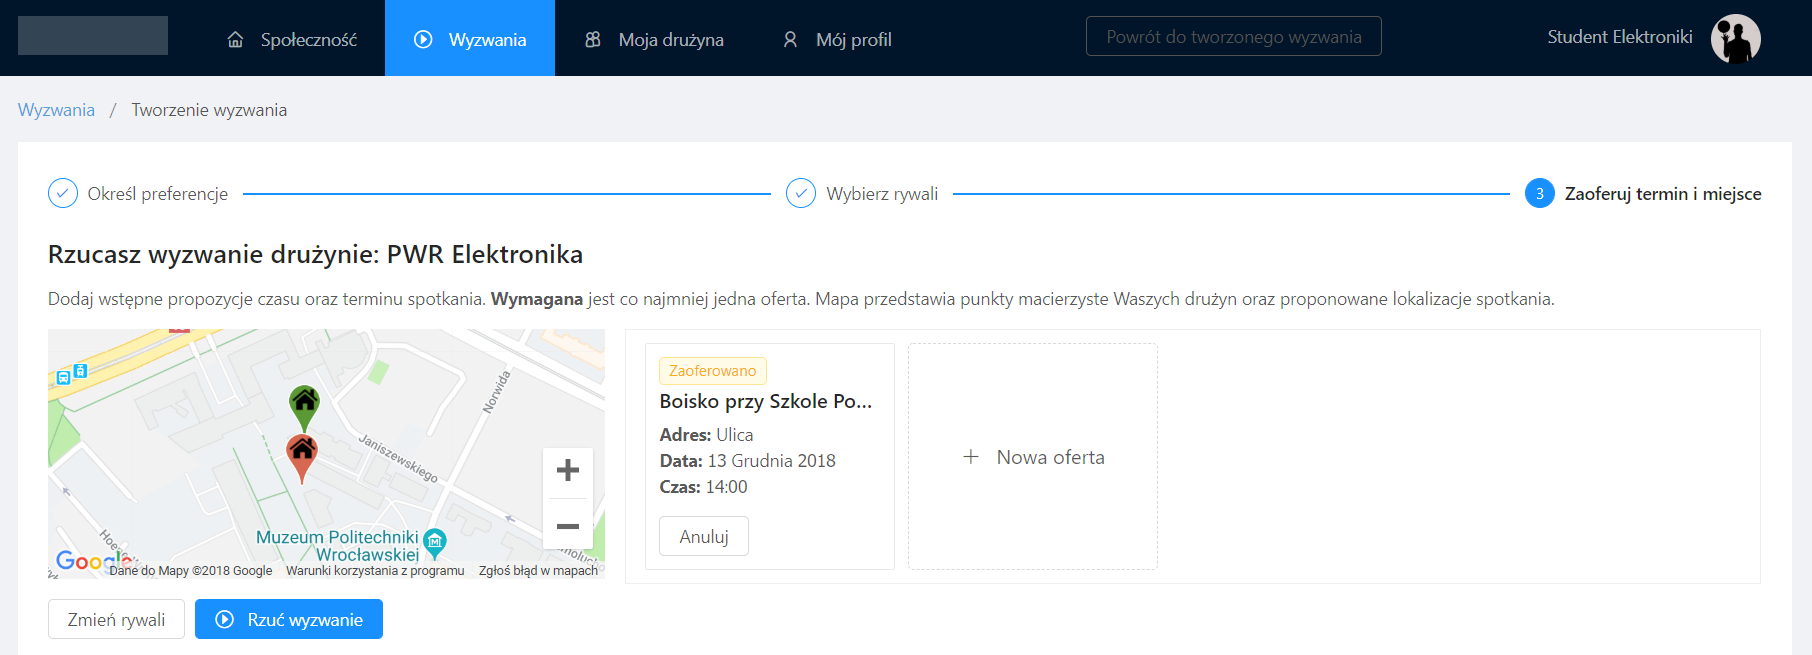
\includegraphics[width=\linewidth]{065-dzialanie/rys/ss-search-7.PNG}
\caption{Widok zaktualizowanej puli wstępnych ofert czasu oraz miejsca spotkania}
\label{fig:ss-search-7}
\end{figure}


W wyniku rzucenia wyzwania zostaje ono zarejestrowane w systemie oraz od tej pory jest widoczne w zakładce ``Wyzwania``. Początkowym stanem każdego nowego wyzwania są negocjacje. Szczegóły dotyczące tego procesu zostaną opisane w następnej części tego rozdziału. Widok obecnych wyzwań został przedstawiony na rysunku \ref{fig:ss-search-8}.

\begin{figure}[H]
\centering
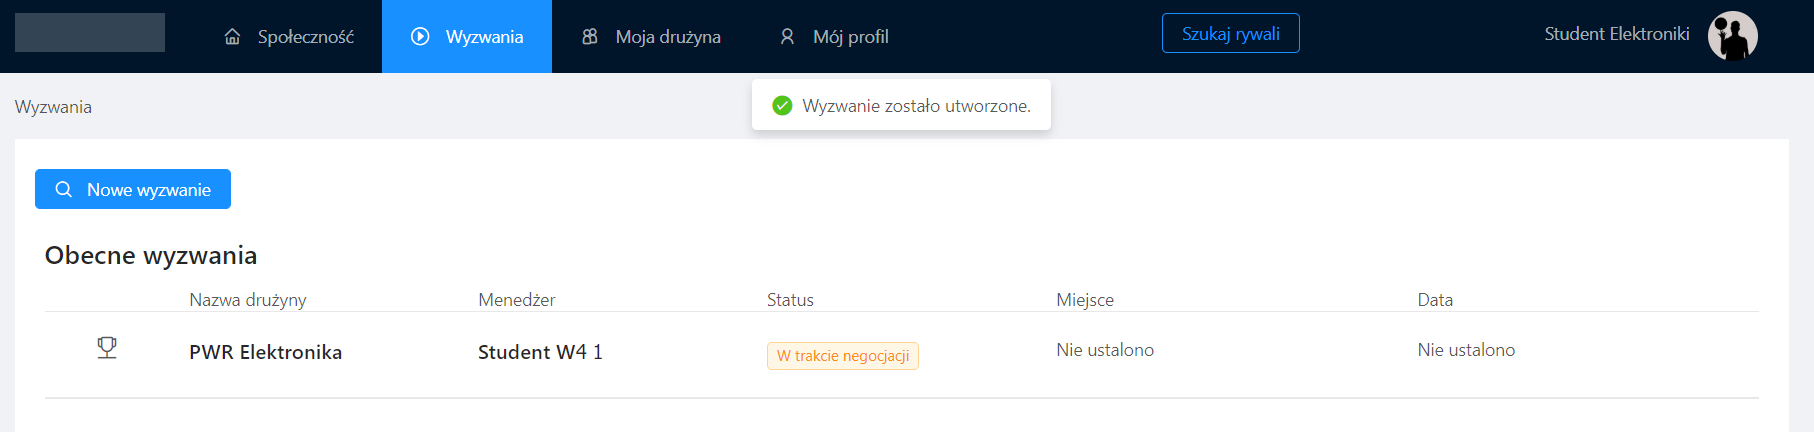
\includegraphics[width=\linewidth]{065-dzialanie/rys/ss-search-8.PNG}
\caption{Widok obecnych wyzwań}
\label{fig:ss-search-8}
\end{figure}


\section{Umawianie spotkań i wprowadzanie wyników}

Umawianie spotkań jest ważną funkcjonalnością prowadzącą do realizacji celów systemu, czyli zrzeszania zawodników. Widok obecnych oraz zakończonych wyzwań przedstawiono na rysunku \ref{fig:ss--match-0}. Aktualne wyzwanie jest w stanie negocjacji. Dodatkowo widać informacje o istnieniu ofert czasu i miejsca od rywali, które nie zostały rozpatrzone - odrzucone bądź zaakceptowane.

\begin{figure}[H]
\centering
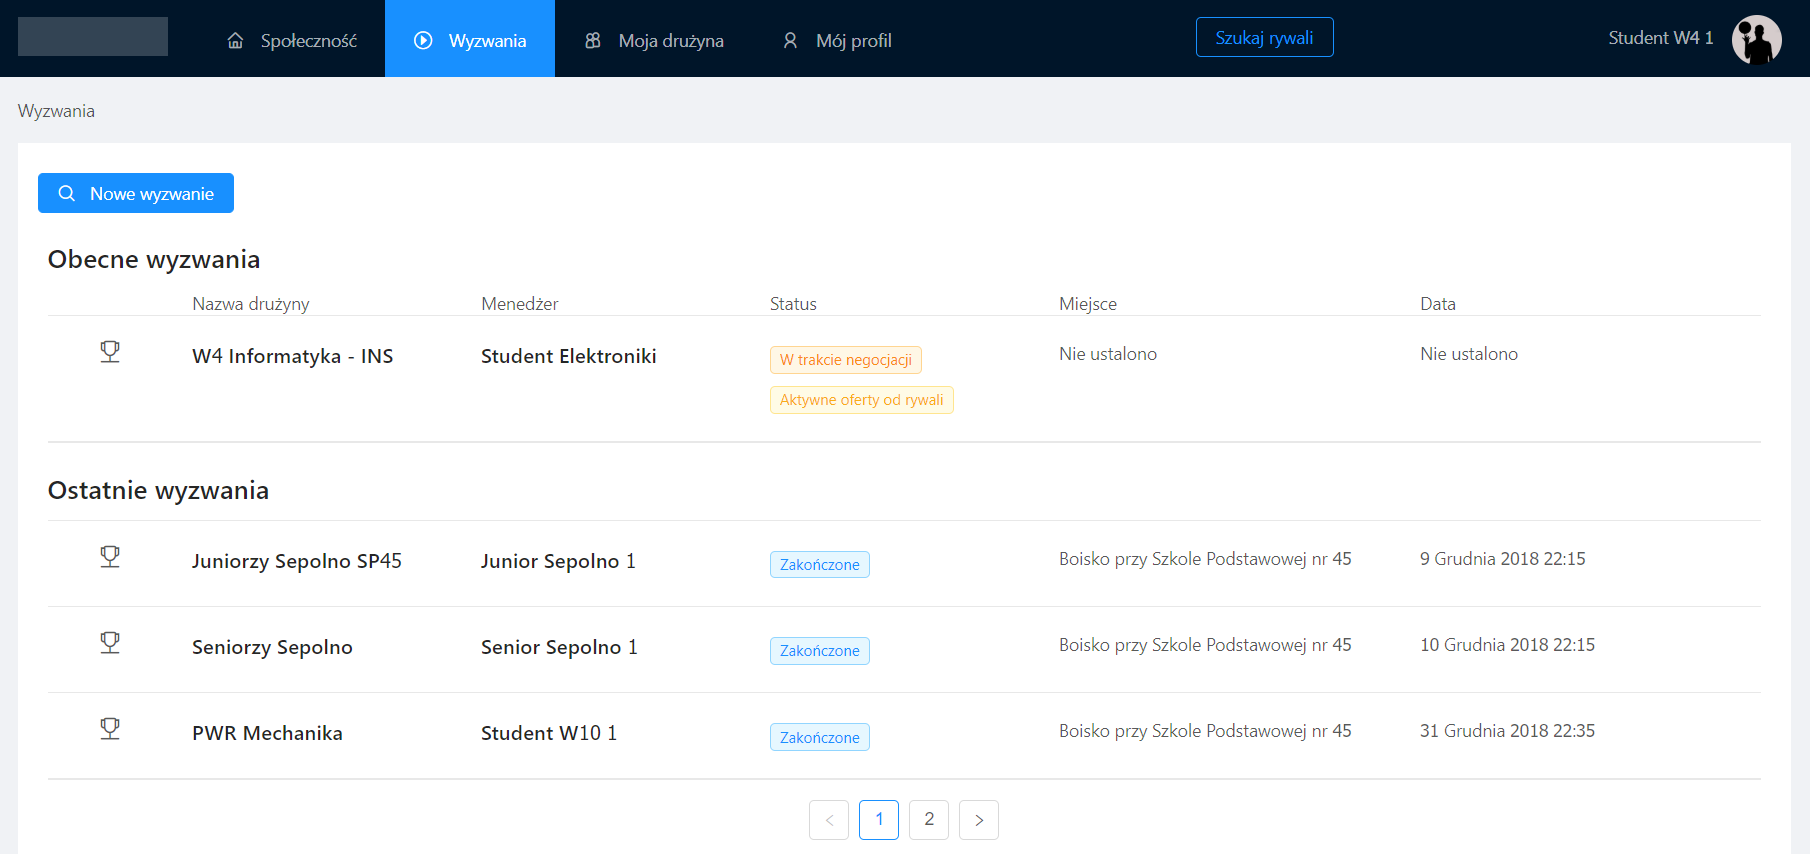
\includegraphics[width=\linewidth]{065-dzialanie/rys/ss-match-0.PNG}
\caption{Widok zakładki ``Wyzwania``}
\label{fig:ss--match-0}
\end{figure}

Użytkownik może wejść w szczegóły poszczególnych wyzwań klikając na nie. Po wykonaniu tej czynności ukazuje się widok przedstawiony na rysunku \ref{fig:ss--match-1}. Widok ten prezentuje dodatkowe informacje na temat wyzwania, a także umożliwia podejmowanie akcji.

\begin{figure}[H]
\centering
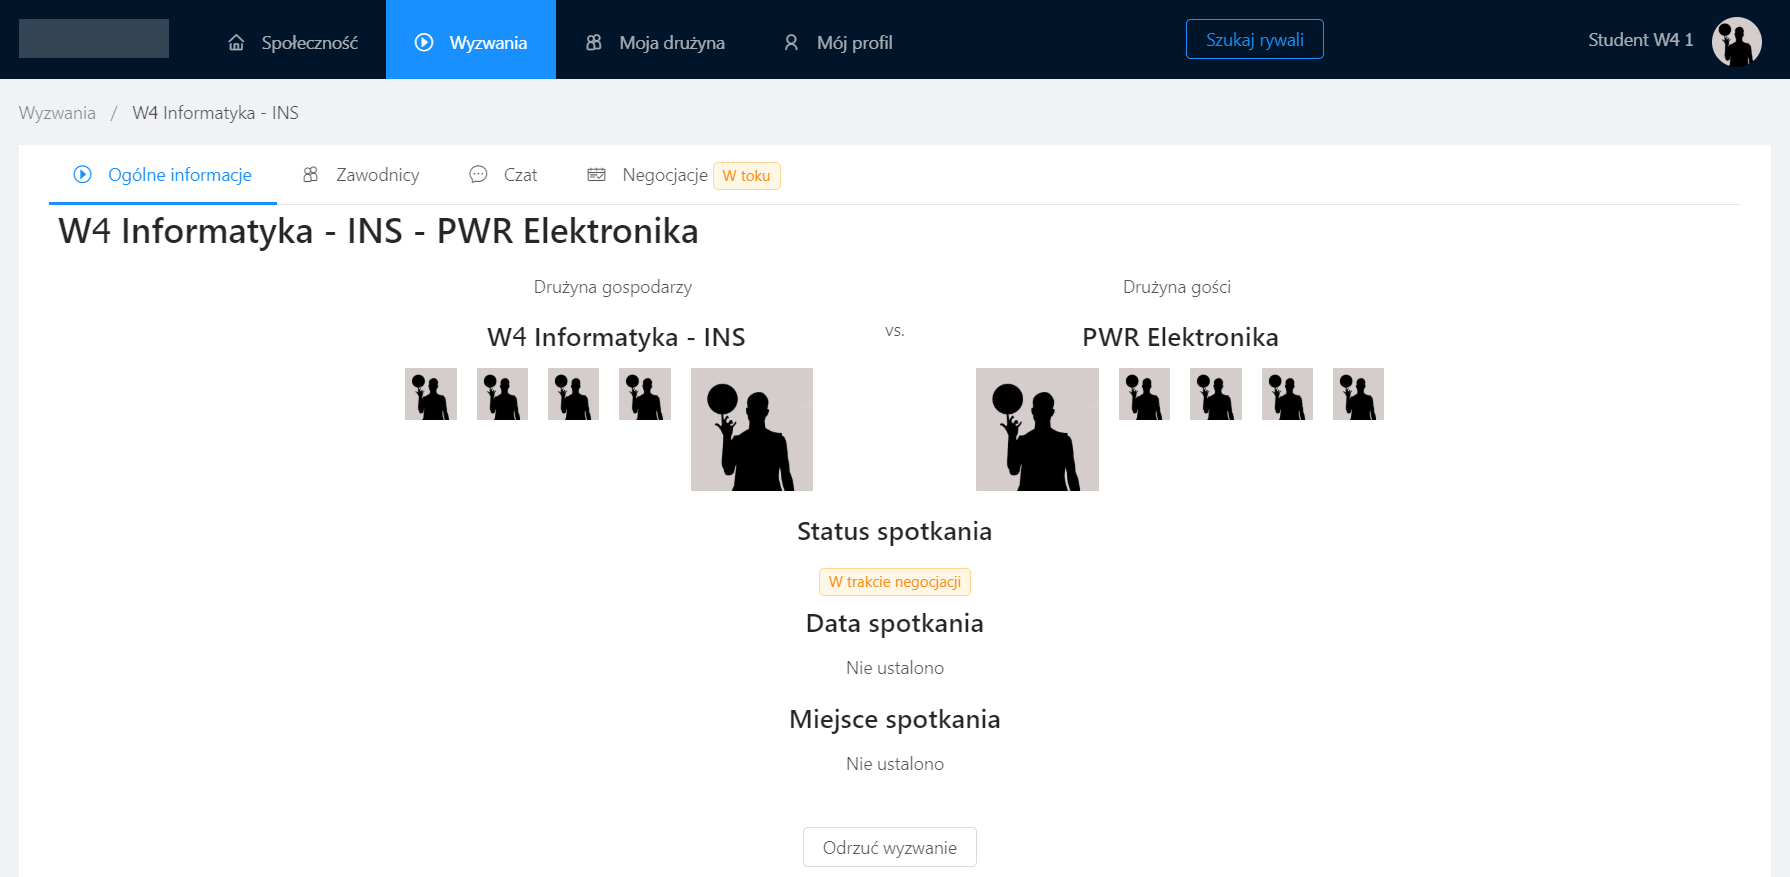
\includegraphics[width=\linewidth]{065-dzialanie/rys/ss-match-1.PNG}
\caption{Widok szczegółów wybranego wyzwania w trakcie negocjacji}
\label{fig:ss--match-1}
\end{figure}

Po utworzeniu wyzwania szczególnie ważny jest widok negocjacji, który został przedstawiony na rysunku \ref{fig:ss--match-2}. Po lewej stronie znajdują się oferty czasu i miejsca spotkania aktywnej drużyny oraz jej rywali. Kapitan może wprowadzać nowe oferty, anulować swoje, bądź odrzucać i akceptować oferty rywali. Akceptacja oferty rywali równoznaczna jest ze zgodą obydwu drużyn na powiązane z nią miejsce oraz czas spotkania. 

\begin{figure}[H]
\centering
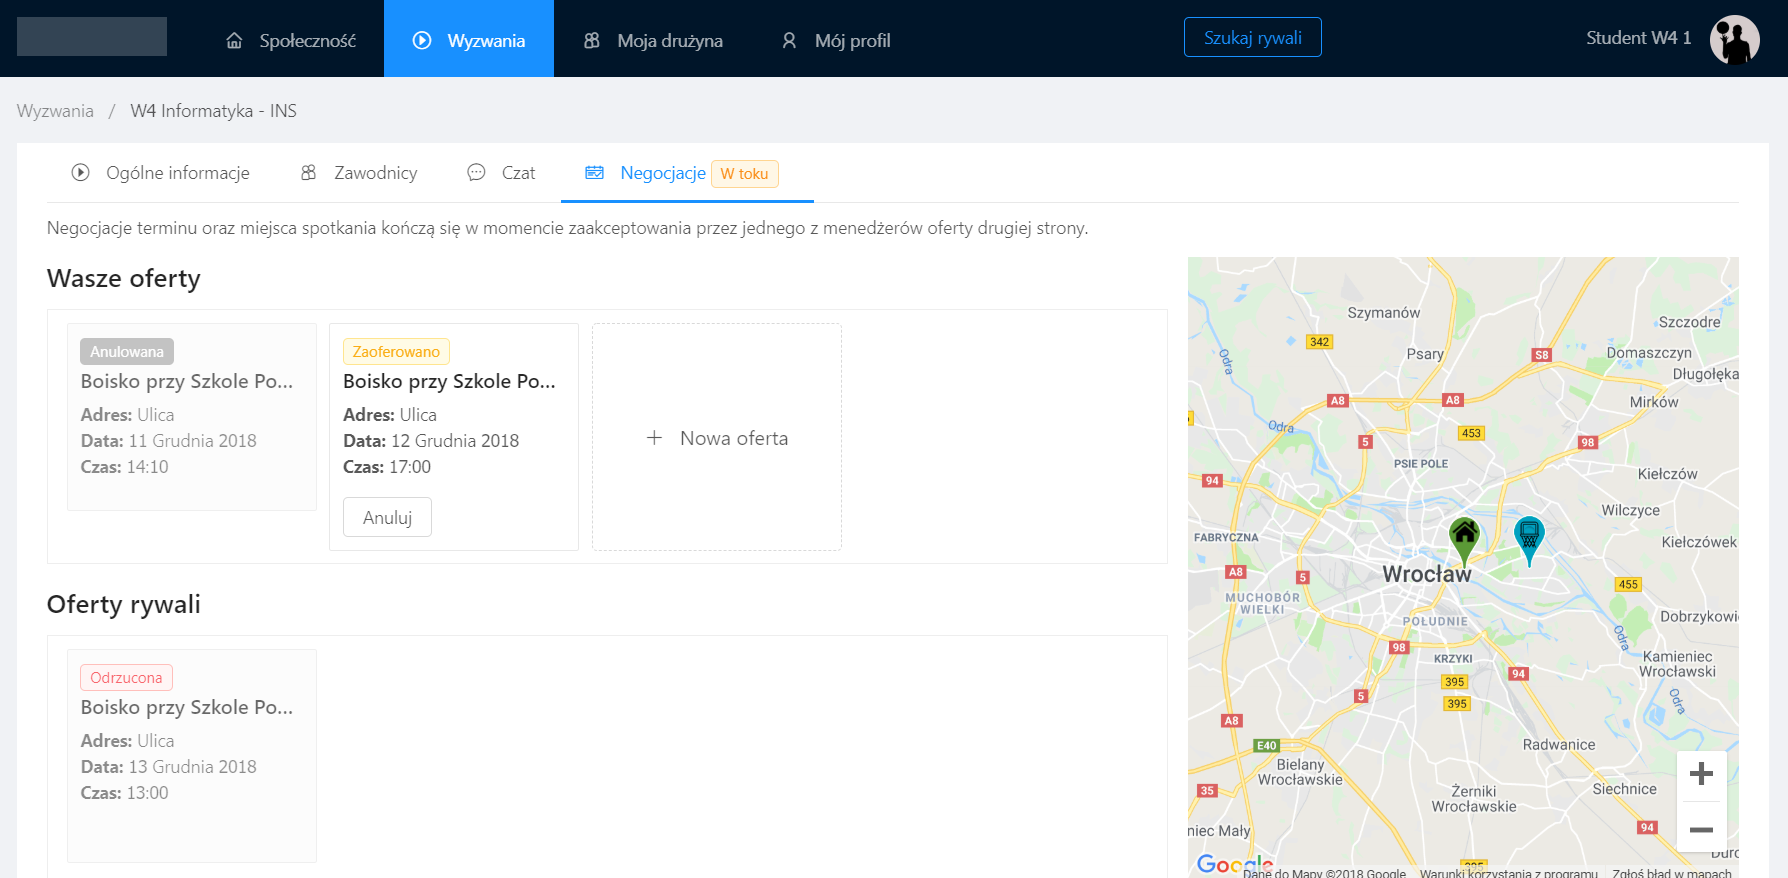
\includegraphics[width=\linewidth]{065-dzialanie/rys/ss-match-2.PNG}
\caption{Widok negocjacji miejsca oraz czasu spotkania - w trakcie negocjacji}
\label{fig:ss--match-2}
\end{figure}

Na rysunku \ref{fig:ss--match-3} przedstawiono widok po uzyskaniu zgody obydwu drużyn. Pozostałe oferty są automatycznie odrzucane, a proces negocjacji kończy się. Widok zaktualizowanych szczegółów spotkania wraz z jego ustaloną datą oraz miejscem przedstawiono na rysunku \ref{fig:ss--match-4}.

\begin{figure}[H]
\centering
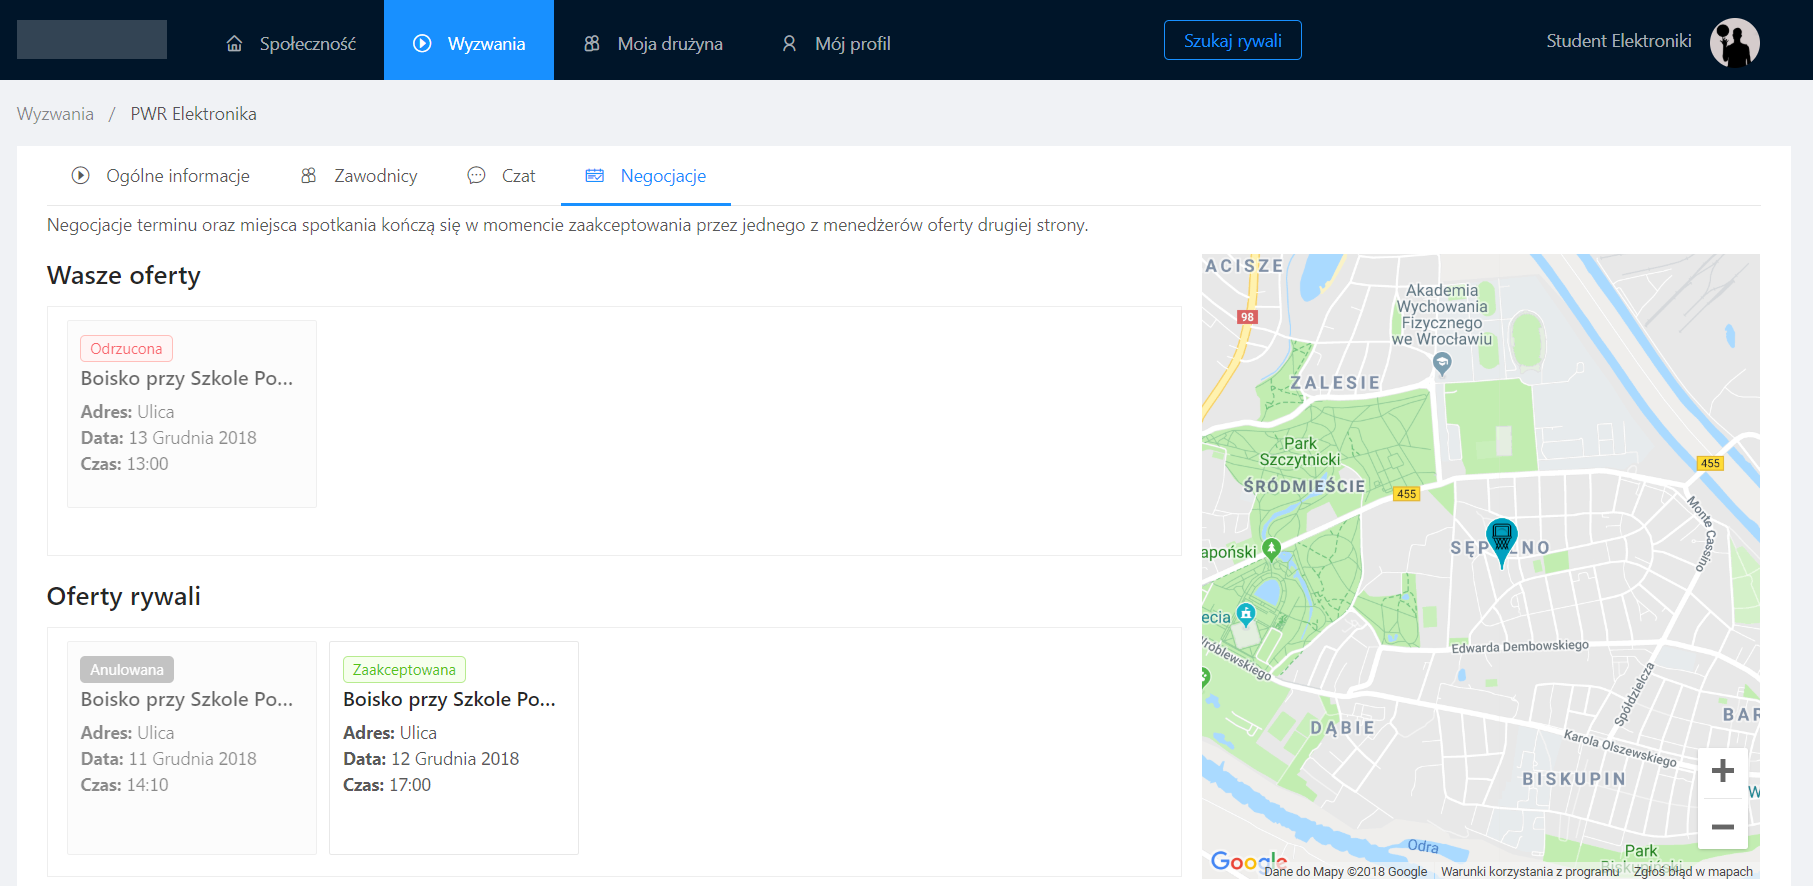
\includegraphics[width=\linewidth]{065-dzialanie/rys/ss-match-3.PNG}
\caption{Widok negocjacji miejsca oraz czasu spotkania - po zaakceptowaniu}
\label{fig:ss--match-3}
\end{figure}

\begin{figure}[H]
\centering
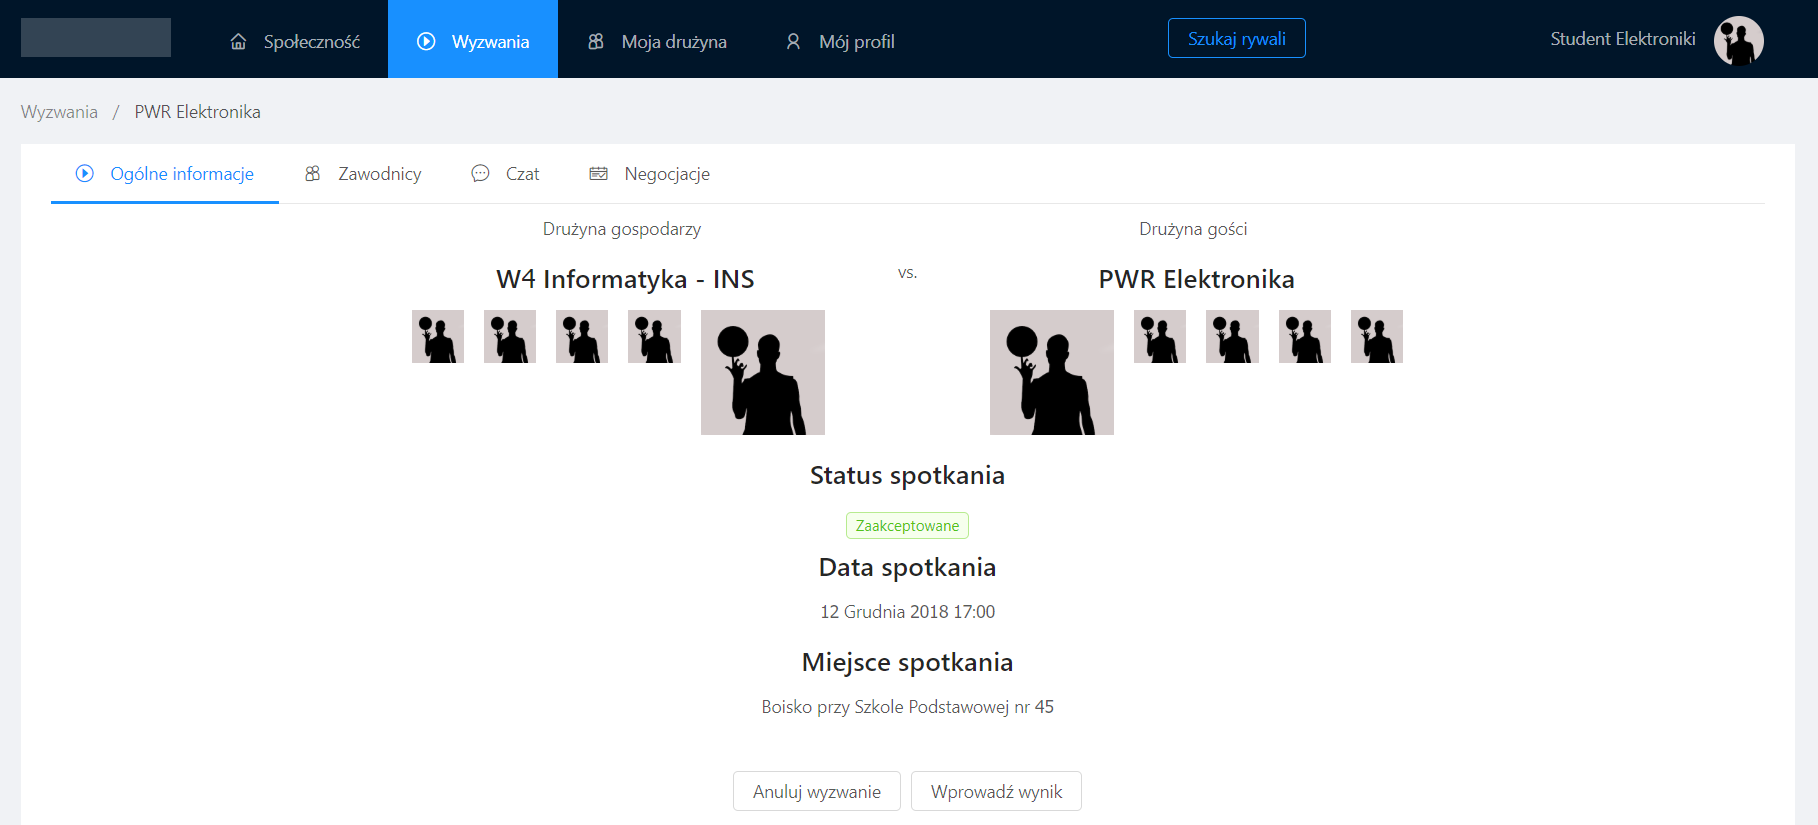
\includegraphics[width=\linewidth]{065-dzialanie/rys/ss-match-4.PNG}
\caption{Widok szczegółów zaakceptowanego wyzwania}
\label{fig:ss--match-4}
\end{figure}

W celu sfinalizowania wyzwania po jego rozegraniu drużyny powinny wprowadzić do systemu wynik meczu. Obojętnie który z kapitanów może w tym celu użyć przycisku ``Wprowadź wynik`` dostępnego dla wyzwań w stanie ``Zaakceptowane``. Wyświetlane jest okno dialogowe przedstawione na rysunku \ref{fig:ss--match-6}. Kapitan wprowadza punkty zdobyte przez poszczególne drużyny. Symbol pucharu umieszczany jest automatycznie nad drużyną, która zdobyła więcej punktów.

\begin{figure}[H]
\centering
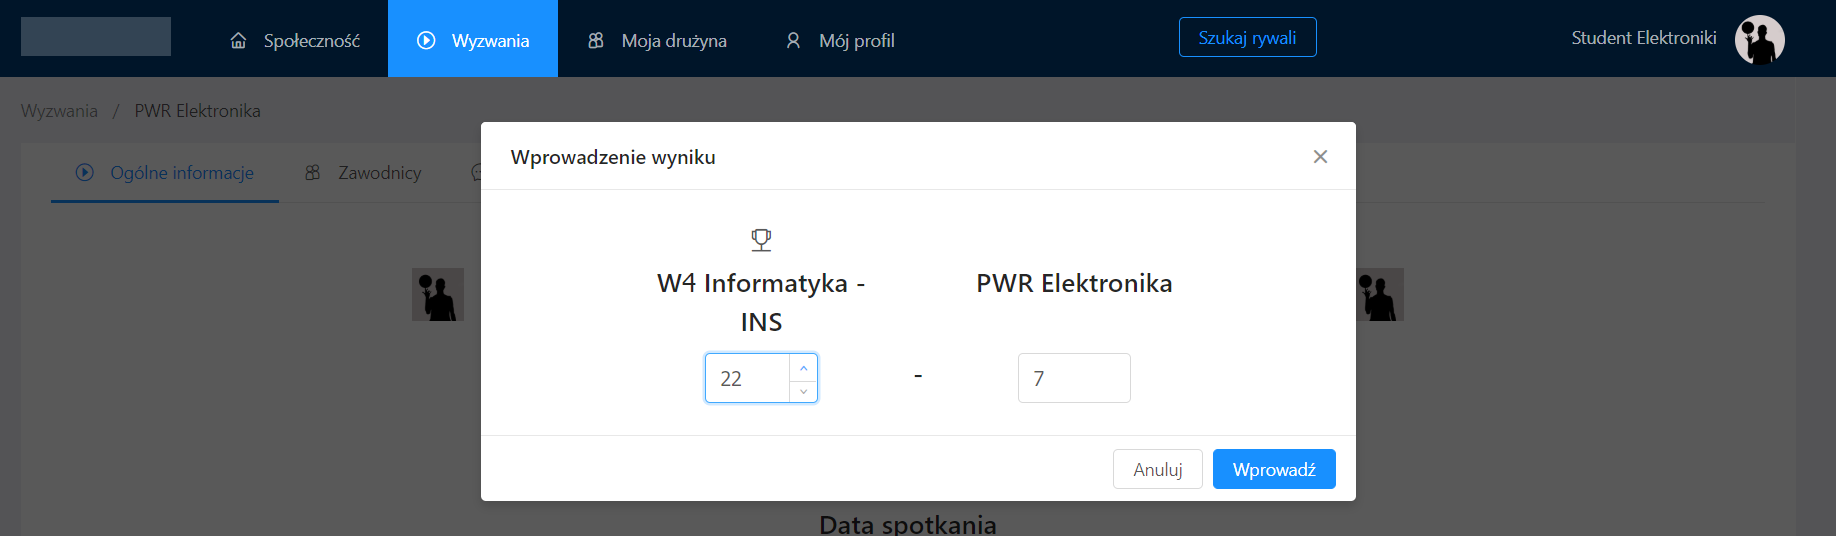
\includegraphics[width=\linewidth]{065-dzialanie/rys/ss-match-6.PNG}
\caption{Widok formularza wprowadzania wyniku wyzwania}
\label{fig:ss--match-6}
\end{figure}

\begin{figure}[H]
\centering
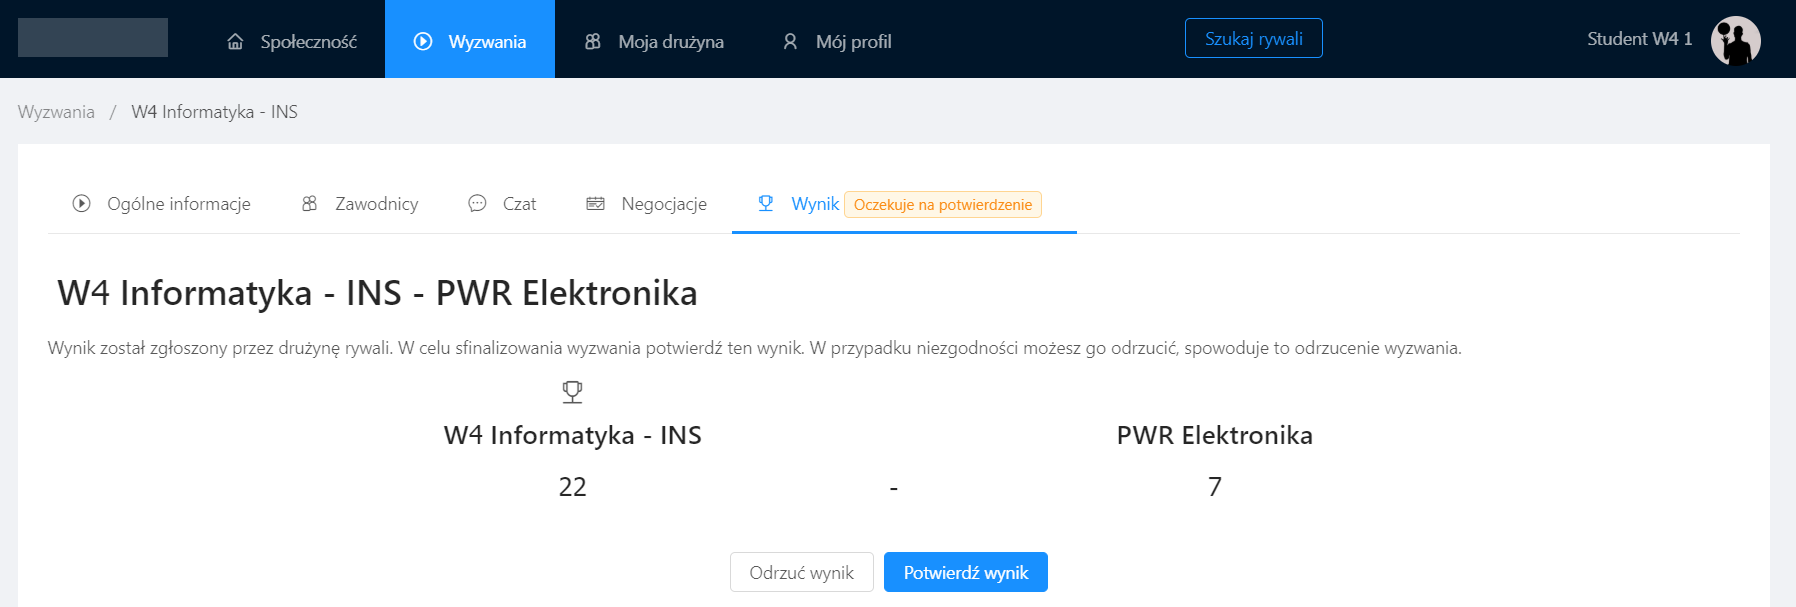
\includegraphics[width=\linewidth]{065-dzialanie/rys/ss-match-8.PNG}
\caption{Widok zakładki ``Wynik`` w przypadku niezaakceptowanego wyniku}
\label{fig:ss--match-8}
\end{figure}

Wprowadzony wynik musi zostać potwierdzony przez drugiego z kapitanów lub odrzucony w przypadku niezgodności, co przedstawiono na rysunku \ref{fig:ss--match-8}. W momencie uzyskania zgody obydwu kapitanów odnośnie rezultatu spotkania zostaje ono oznaczone jako zakończone. Widok zaktualizowanego wyzwania przedstawiono na rysunku \ref{fig:ss--match-9}.

\begin{figure}[H]
\centering
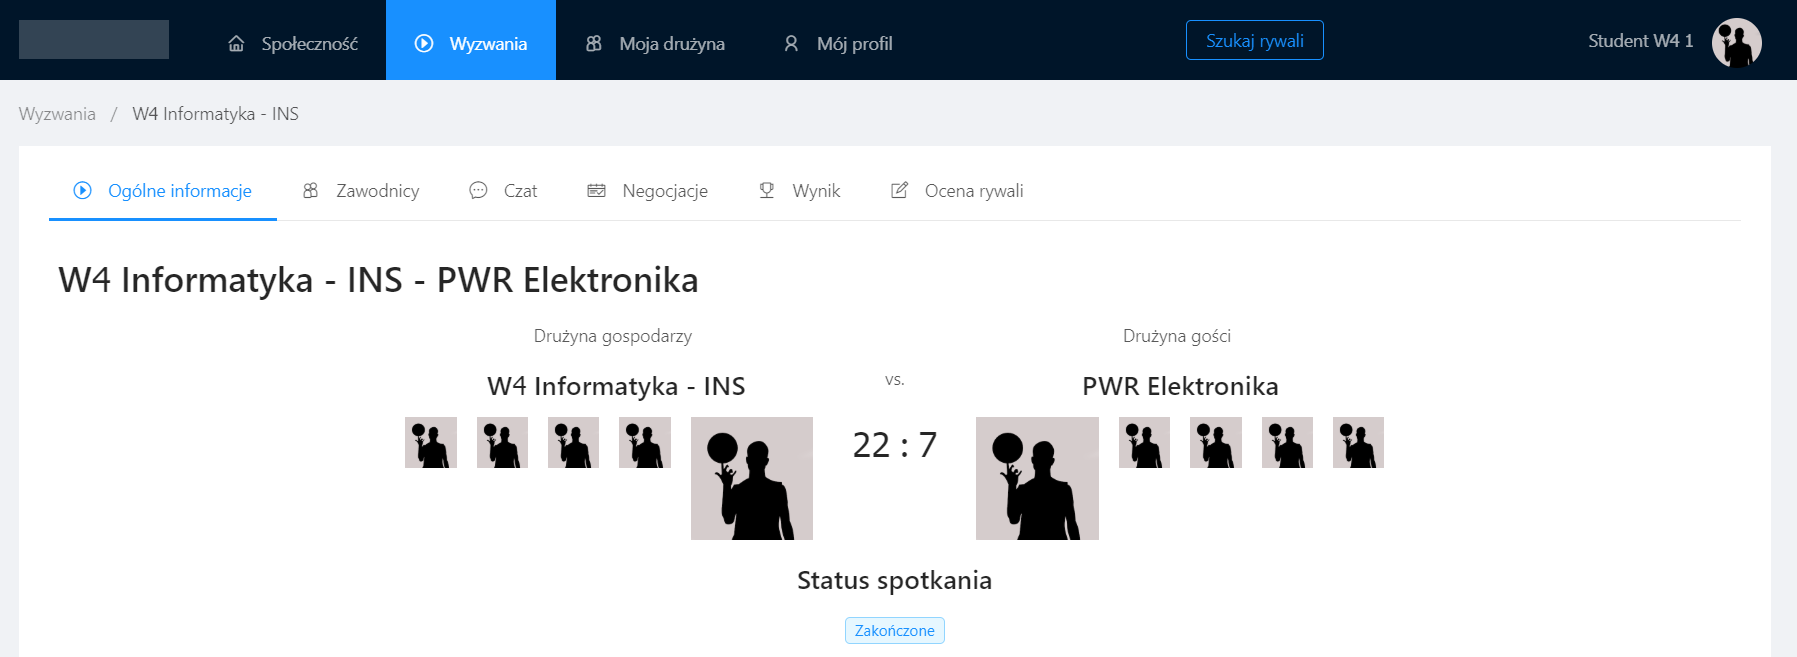
\includegraphics[width=\linewidth]{065-dzialanie/rys/ss-match-9.PNG}
\caption{Widok szczegółów zakończonego wyzwania}
\label{fig:ss--match-9}
\end{figure}

Ostatnim krokiem jaki kapitanowie drużyn mogą podjąć w ramach wyzwania jest ocenienie rywali. Formularz oceny został przedstawiony na rysunku \ref{fig:ss--match-10}. Przesłanie formularza jest opcjonalne, jednak ma duży wpływ na działanie systemu. Drużyny oceniane wysoko pod względem poziomu fair-play są wyróżniane w wynikach wyszukiwania specjalnym znacznikiem. W przypadku deklaracji chęci ponownego spotkania drużyna będzie oznaczona znacznikiem ``Zagraj ponownie``, ale tylko dla drużyny, która wyraziła taką chęć.

\begin{figure}[H]
\centering
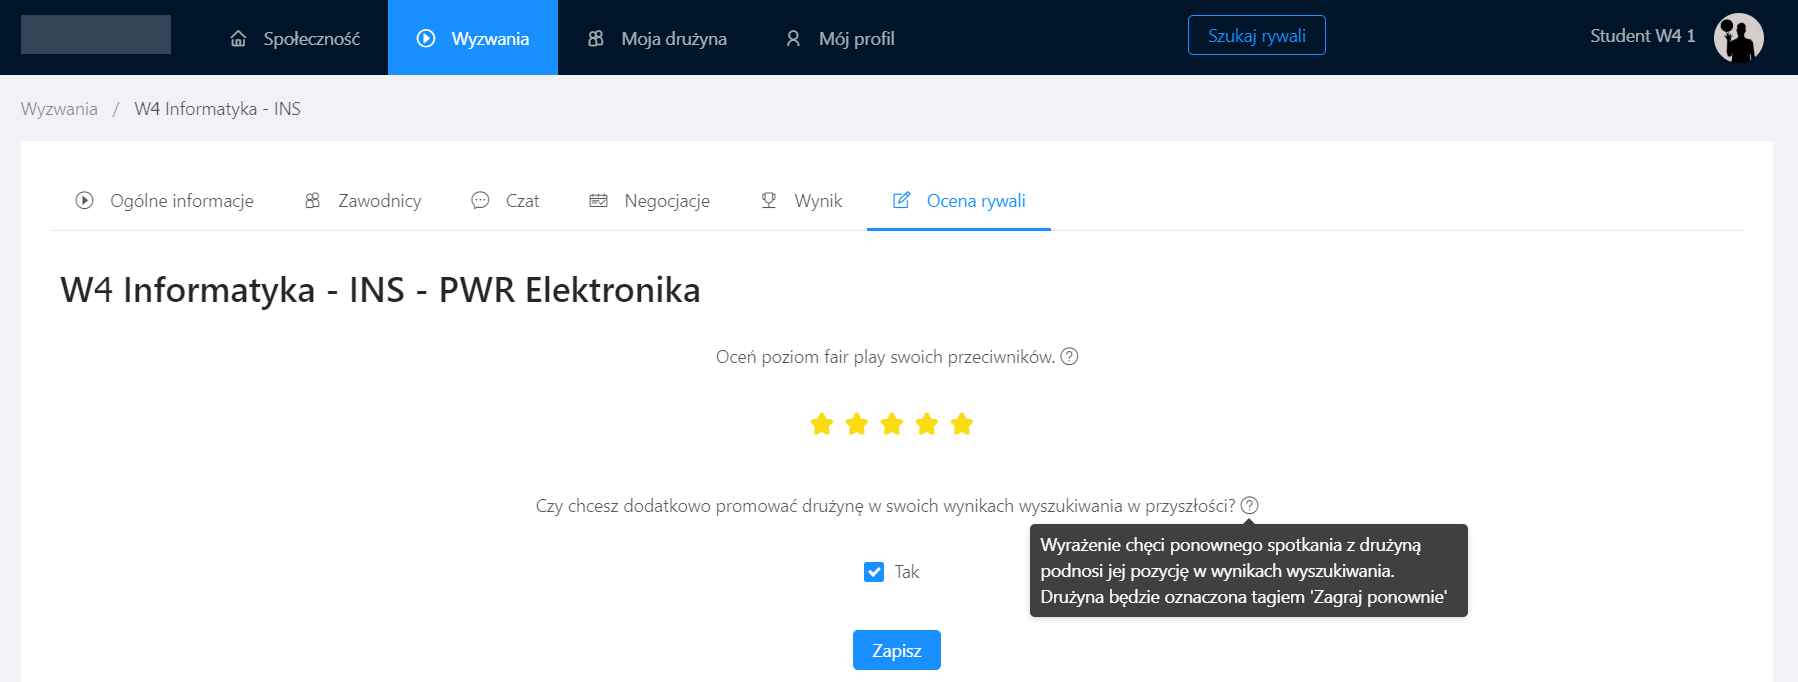
\includegraphics[width=\linewidth]{065-dzialanie/rys/ss-match-10.PNG}
\caption{Widok formularza oceny rywali}
\label{fig:ss--match-10}
\end{figure}
